\documentclass[11pt,onecolumn]{IEEEtran}
\usepackage{amsmath,amssymb,amsthm}
\usepackage{graphicx}
\usepackage{tikz}
\usepackage[hidelinks]{hyperref}

\newtheorem{theorem}{Theorem}
\newtheorem{proposition}[theorem]{Proposition}
\newtheorem{corollary}[theorem]{Corollary}
\newtheorem{lemma}[theorem]{Lemma}
\newtheorem{remark}[theorem]{Remark}
\newtheorem{definition}[theorem]{Definition}

\newcommand{\E}{\mathbb{E}}
\newcommand{\R}{\mathbb{R}}
\newcommand{\tr}{\operatorname{tr}}
\newcommand{\Cov}{\operatorname{Cov}}
\newcommand{\cX}{\mathcal{X}}
\newcommand{\hX}{\widehat{X}}
\newcommand{\hXn}{\widehat{X}^{n}}
\newcommand{\hY}{\widehat{Y}}
\newcommand{\RW}{\mathcal{R}\!\mathcal{W}}
\newcommand{\Bdet}{\mathsf{B}_{\det}}
\newcommand{\LRs}{L_{R}^{\star}}
\newcommand{\RLs}{R_{L}^{\star}}
\newcommand{\kb}{k_{\mathrm{B}}}

\begin{document}

\title{Tradeoffs Between Rate and Conditional Content\\ with Encoder-Observed Context}

\author{Andrew~H.~Bond,~\IEEEmembership{Senior Member,~IEEE}%
\thanks{A. H. Bond is with the Department of Computer Engineering, San Jos\'e
State University, San Jos\'e, CA 95192 USA (e-mail: andrew.bond@sjsu.edu).
Numerical verification harnesses and archived records:
\url{https://github.com/ahb-sjsu/geometric-observation}; this manuscript, its full-length versions, and its verification scripts are archived at doi:10.5281/zenodo.22678342.}}

\markboth{IEEE Transactions on Information Theory}{Bond: Tradeoffs Between Rate and Conditional Content with Encoder-Observed Context}

\maketitle

\begin{abstract}
An encoder observes a jointly Gaussian pair $(Y,V)$ and describes $Y$ at rate
$R$ for a decoder that sees the description alone; the correlated variable
$V$ is the context. A third party retains a noisy copy $S=V+U$ of the
context and never decodes. We characterize the conditional content
$L=I(X;\hX\mid S)$ of the stored description relative to the retained
context: Steinberg's common-reconstruction functional applied to the
augmented source $X=(Y,V)$ with distortion on $Y$ alone. In the
average-work form of Landauer's bound with side information, $L$ is
exactly the ideal erasure work per symbol in units of $\kb T\ln 2$.
Three results are primary. First, a closed form:
$L(D)=\tfrac12\log_2 g^\star$, with $g^\star$ the larger root of an
explicit quadratic whose coefficients are set by $(D,\rho^2,\tau^2)$, when
$Y$ and $V$ are scalar linear functionals of an arbitrary-dimensional
jointly Gaussian source. Second, the exact rate--content region: its
Pareto frontier is a coupled two-water-level system, nondegenerate exactly
when $0<\rho^2<1$ within the strictly noisy model $\tau^2>0$, with the
strict tradeoff persisting at the clean-context boundary. Third,
non-determination: two instances whose $(Y,S)$ laws are equivalent up to
bijective scaling have different $L$, so replacing the encoder's
observation of $(Y,V)$ by its reduced relation to $S$ changes the
operational problem, and the augmentation is essential. The closed form
recovers the classical rate--distortion function at $\rho=0$ and Gray's
conditional function as $\tau^2\to0$, and meets Steinberg's scalar
Gaussian formula as $\rho^2\to1$. We also record exactly when the
natural determinant lower bound is attained, and give the joint
rate--content frontier of the doubly symmetric binary case through a tilt
equation anchored at Gray's function and the marginal rate--distortion
function.
\end{abstract}

\begin{IEEEkeywords}
Rate--distortion theory, side information, common reconstruction, conditional
mutual information, Gaussian sources.
\end{IEEEkeywords}

\section{Introduction}
\label{sec:intro}

A stored description of data has two prices. The first is its rate, the space
the description occupies, and rate--distortion theory prices it against the
fidelity the decoder requires. The second is paid at the end of the
description's life: erasing a stored description irreversibly costs work, and
when the mechanism performing the reset retains correlated information, the
work is governed not by the description's entropy but by its conditional
entropy given what the mechanism holds. The two prices are set by different
parties. The decoder never sees the reset mechanism's information, and the
reset mechanism never serves the decoder. This paper solves the source coding problem that this
asymmetry creates, for Gaussian and binary sources, in closed form.

The setting is as follows. An encoder observes a jointly Gaussian pair
$(Y,V)$: $Y$ is the variable the decoder must reproduce, and $V$ is a
correlated variable, which we call the context ($\rho=\E[YV]$ after
normalization). The encoder emits a description under a distortion constraint
$\E(Y-\hY)^2\le D$ that binds the unconditional error; the decoder
reconstructs from the description alone. A third
party holds $S=V+U$, a noisy observation of the context with noise variance
$\tau^2$. The quantity of interest is
$L(D)=\min I(X;\hX\mid S)$ over test channels satisfying the distortion
constraint and the Markov chain $\hX-X-S$. We call $L(D)$ the minimal
conditional content of an admissible description; by the operational
theorems of Section~\ref{sec:operational} and, for the Gaussian source,
Appendix~\ref{app:gaussian}, it is the least asymptotically achievable
value of the normalized conditional entropy $H(M\mid S^n)/n$ of the stored
index $M$ among codes meeting the distortion constraint. The
thermodynamic reading of this quantity, as the minimal average erasure
work per symbol under an ideal conditional reset, is stated once, in
Remark~\ref{rem:thermo}, together with the setting it needs.

The single-letter functional itself is not new. With the augmented source
$X=(Y,V)$ and a distortion that ignores the $V$ coordinate,
$\min I(X;\hX\mid S)$ is exactly Steinberg's common-reconstruction
functional \cite{steinberg2009}, and Remark~8 of Lapidoth, Mal\"ar, and
Wigger \cite{lapidoth2014} notes precisely this augmentation device: an
encoder observing an additional sequence correlated with the side
information is handled by enlarging the source alphabet and letting the
distortion ignore the extra coordinate. What this paper adds is the
solution of the augmented problem, and three contributions are primary.
First, the closed form: we evaluate the augmented Gaussian functional
exactly, $L(D)=\tfrac12\log_2 g^\star$ with $g^\star$ the larger root of
an explicit quadratic together with the achieving channel
(Theorem~\ref{thm:function}), after Theorem~\ref{thm:pair} reduces the
problem, for $Y$ and $V$ scalar linear functionals of an
arbitrary-dimensional jointly Gaussian source, to the pair
$(\rho,\tau^2)$. The known Gaussian solutions are scalar and
unaugmented: Steinberg's Gaussian example \cite{steinberg2009} and the
Gaussian theorem of \cite{lapidoth2014} take a scalar source with side
information $X+U$ and an encoder that observes the source alone, and
the augmentation remark of \cite{lapidoth2014} is stated for finite
alphabets, so the augmented Gaussian functional is evaluated in
neither. Second, the
exact rate--content region with its strict misalignment dichotomy: the
Pareto frontier is traced by a coupled two-water-level stationarity
system, and within the strictly noisy model $\tau^2>0$ it is
nondegenerate, so that rate and content strictly trade off, exactly when
$0<\rho^2<1$, with the tradeoff persisting at the clean-context boundary
(Theorem~\ref{thm:region} and Corollary~\ref{cor:misalign}). Third,
non-determination by the reduced marginal
(Corollary~\ref{cor:notmarginal}): replacing the encoder's observation of
the pair $(Y,V)$ by its reduced relation to $S$ changes the operational
problem even when the reduced $(Y,S)$ laws are equivalent up to invertible
scaling. That is the one-line answer to why the function is not
Steinberg's scalar formula: the encoder's access to the clean context
$V$, which neither the decoder nor the third party shares, enters the
function itself. The operational layer supports these results rather than
leading them: coding theorems characterize $L(D)$ as the least
asymptotically achievable normalized conditional entropy $H(M\mid S^n)/n$
of the stored index (Section~\ref{sec:operational}, and
Appendix~\ref{app:gaussian} for the Gaussian source), and the
thermodynamic reading of $L(D)$ (Remark~\ref{rem:thermo}) is one
consequence of that characterization.

More broadly, the problem shows that the operational content of a
description need not be an intrinsic property of the description alone.
It can depend on the configuration in which the description is observed:
the information available to the encoder, the distortion criterion the
decoder imposes, and the correlated context another party retains. The
non-determination result makes this dependence exact within the present
model. The reduced source--context relation does not determine the
conditional-content cost, because the encoder's observational access
itself enters the problem. In the vocabulary of \cite{bond2026landauer},
the content is consumer-relative.

The remaining results are structural consequences, extensions, and
consistency anchors. Remark~\ref{rem:floor} records, with the proof
deferred to the archived full-length version, when the natural
determinant lower bound is attained: the attainment condition involves
the encoder-accessible conditional covariance, not the third party's.
Three extensions follow: the binary
case closes completely, for a doubly symmetric binary source with a
binary symmetric context channel, through an elementary tilt equation
anchored at Gray's binary conditional function and the marginal
rate--distortion function (Section~\ref{sec:binary}); the frontier
extends to vector context (Section~\ref{sec:vector}); and the operational
region theorem is proved directly for the Gaussian source
(Appendix~\ref{app:gaussian}). The consistency anchors are the three
classical corners of the closed form, Shannon's rate--distortion function
at $\rho=0$ \cite{shannon1959}, Gray's conditional function as
$\tau^2\to0$ \cite{gray1973}, and Steinberg's scalar Gaussian formula at
the induced correlation as $\rho^2\to1$, together with the strict
suboptimality of marginalization and an exact information-bottleneck
identity for the weighted objective.

\subsection*{Relation to prior formulations}

Table~\ref{tab:whatsnew} places each main result against its nearest
published neighbor. The single-letter functional is inherited: it is
Steinberg's common-reconstruction functional \cite{steinberg2009},
applied unchanged to the augmented source. The augmentation device is
also inherited, as Remark~8 of \cite{lapidoth2014}. What is contributed
is the evaluation of the reduced problem; the closed form, the two
coupled water levels, the misalignment dichotomy, and the
non-determination phenomenon of Corollary~\ref{cor:notmarginal} are
properties of the solution rather than of the reduction. The physical
reading leaves the mathematics unchanged: the coordinate
$H(M\mid S^n)/n$ is characterized by a proved coding theorem
(Section~\ref{sec:operational} and Appendix~\ref{app:gaussian}), and
the thermodynamic reading is confined to Remark~\ref{rem:thermo}, one
consequence of that theorem. The proof
machinery is classical, but the solved augmented optimization and its
joint region are, to our knowledge, new: we are unaware of a prior
derivation of this particular coupled frontier, in which two levels are
tied by a common distortion constraint, and the quadratic of
Section~\ref{sec:function} does not appear in the literature we surveyed.
Figure~\ref{fig:frontiermulti} shows the resulting tradeoff at three
correlations.

\begin{table}[!t]
\caption{Theorem-level comparison with the nearest prior results.}
\label{tab:whatsnew}
\centering
\footnotesize
\begin{tabular}{p{1.35in}p{1.55in}p{1.55in}p{1.55in}}
\hline
Result here & Nearest prior & What the prior establishes & What is new
here\\
\hline
Closed form (Theorem~\ref{thm:function}) & Steinberg
\cite{steinberg2009}; Lapidoth--Mal\"ar--Wigger \cite{lapidoth2014} &
Scalar Gaussian CR formula; scalar Gaussian theorem with side
information $X+U$, encoder observing the source alone; the augmentation
remark stated for finite alphabets & The augmented source
$(Y,V)$, with $Y$ and $V$ scalar linear functionals of an
arbitrary-dimensional source; the quadratic $g^\star$; the achieving
channel\\
Rate--content region (Theorem~\ref{thm:region}) & \cite{steinberg2009,
lapidoth2014}; Gaussian IB \cite{chechik2005} & Rate under a CR
constraint; unconstrained IB Lagrangian with its eigenmode structure &
The joint $(R,L)$ region; a two-water-level frontier under a hard
distortion constraint\\
Misalignment dichotomy (Corollary~\ref{cor:misalign},
Remark~\ref{rem:cleanboundary}) & none known to us & & Strict tradeoff iff
$0<\rho^2<1$ under $\tau^2>0$; persistence at $\tau^2=0$\\
Non-determination by the reduced marginal
(Corollary~\ref{cor:notmarginal}) & Remark~8 of \cite{lapidoth2014} &
The augmentation reduction exists & The value depends strictly on the
augmentation: same $(Y,S)$ law up to bijective scaling, different $L$\\
Binary function (Theorem~\ref{thm:binary}) & Lu \emph{et al.}
\cite{lu2016lossy,lu2016binary}; Steinberg \cite{steinberg2009}; Ahmadi et
al. \cite{ahmadi2013} & The DSBS common-reconstruction rate, which equals our
$L(D)$ \cite{lu2016lossy}; decoder-SI CR values \cite{steinberg2009,ahmadi2013}
& The joint $(R,L)$ frontier and its tilt parametrization; the $L(D)$ value
itself is inherited from \cite{lu2016lossy} (Appendix~\ref{app:lucompare})\\
\hline
\end{tabular}
\end{table}

\subsection*{Related work}

Conditional rate--distortion theory is due to Gray
\cite{gray1972tr,gray1973}. In that problem both terminals observe the
conditioning variable, and $R_{Y\mid S}(D)$ prices the description under
shared context. Here no terminal observes $S$; Gray's function appears
only as the clean-context limit $\tau^2\to0$ of our function
(Section~\ref{sec:function}). Wyner and Ziv \cite{wynerziv1976} place
the side information at the decoder, where it participates in
reconstruction. Our decoder holds nothing but the description, and
Wyner--Ziv binning enters the operational theorem of
Section~\ref{sec:operational} only as a proof device, through a decoder
that no party in the model operates.

Steinberg \cite{steinberg2009} introduced the common-reconstruction
constraint: the decoder holds side information, but the encoder must be
able to reproduce the decoder's output exactly. The resulting
functional is $\min I(X;\hX\mid S)$ under the Markov chain
$\hX-X-S$, the single-letter object of this paper, and Steinberg
solved its scalar Gaussian case. Lapidoth, Mal\"ar, and Wigger
\cite{lapidoth2014} relaxed exact to approximate reproduction and
solved the Gaussian problem with general jointly Gaussian side
information; their Remark~8 notes that an encoder observing an
additional correlated sequence is incorporated by augmenting the
source and letting the distortion ignore the extra coordinate. Our
problem is exactly that augmented problem, with $X=(Y,V)$ and
distortion on $Y$ alone; Table~\ref{tab:whatsnew} delineates what is
new relative to this line.

Side information held by the encoder alone is classically inert:
when it does not enter the distortion measure, it leaves the
rate--distortion function unchanged \cite{berger1971}. Kaspi
\cite{kaspi1994} analyzed the configurations in which the encoder is
informed of the side information and the decoder may or may not hold
it. In our problem the encoder-held context $V$ matters despite the
classical fact, because the priced coordinate $I(X;\hX\mid S)$ is
conditional on $S$: the encoder never sees $S$, but $V$ is correlated
with it, and access to $V$ strictly lowers the price
(Section~\ref{sec:function}). Heegard and Berger
\cite{heegardberger1985} serve decoders with and without side
information from one description; Ahmadi, Tandon, Simeone, and Poor
\cite{ahmadi2013} imposed the common-reconstruction constraint on the
Heegard--Berger and cascade problems and computed Gaussian and binary
erased-side-information cases. Section~\ref{sec:binary} distinguishes our
binary solution from their calculations and from Steinberg's binary
example.

The Gaussian multi-terminal literature under individual distortion
constraints supplies the exactness anchor of Remark~\ref{rem:floor}:
Xiao and Luo \cite{xiaoluo2005} derived the joint rate--distortion
function of a bivariate Gaussian under individual mean-square
constraints, Lapidoth and Tinguely \cite{lapidothtinguely2010}
re-derived it, and Nayak, Tuncel, G\"und\"uz, and Erkip \cite{nayak2010}
and Stylianou, Charalambous, and Charalambous \cite{stylianou2021}
extended the line to successive refinement and to tuples of vector
sources. These results enter this paper only at one corner of the
attainment condition in Remark~\ref{rem:floor}. The closest
common-reconstruction counterpart is Lu and Xu's vector Gaussian
Heegard--Berger problem with common reconstructions \cite{luxu2021}. Its
rate--distortion function is stated for diagonal positive definite
constraints on every coordinate of the reproduction, and its
achievability is the Timo--Chan--Grant scheme with source enhancement.
The problem here, one decoder and a constraint on the $Y$ coordinate
alone, is the boundary of that setting at which the context coordinate
is unpenalized, outside its stated hypotheses, so
Theorem~\ref{thm:function} is not a specialization of a stated result
of \cite{luxu2021}. We have not derived the closed form from their
expression by a limiting argument; both problems evaluate Steinberg's
functional, so any such extension would have to agree with
Theorem~\ref{thm:function}.

The priced coordinate also has a security reading. Because $L$ is the
normalized conditional entropy $H(M\mid S^n)/n$ of the stored description given
the third party's observation, it is the equivocation of that description at a
party holding the noisy context, and rate--distortion problems under a secrecy
constraint form a long line. Yamamoto priced distortion against the equivocation
of the source in the Shannon cipher system \cite{yamamoto1997}, Villard and
Piantanida characterized secure source coding with side information at the
eavesdropper \cite{villard2013}, and Schieler and Cuff developed a
rate--distortion theory for secrecy systems \cite{schieler2014}. Closer in
form are the side-information-privacy problem of Tandon, Sankar, and
Poor \cite{tandon2013}, which prices the leakage of the description
about the side information against the rate, and the privacy funnel of
Makhdoumi, Salamatian, Fawaz, and M\'edard \cite{makhdoumi2014}, which
minimizes $I(\hX;S)$ at fixed utility. Under the Markov chain the
conditional content is the rate less that leakage,
$I(X;\hX\mid S)=I(X;\hX)-I(\hX;S)$, so the present problem rewards a
description for leaking the context the third party already holds,
since every such bit is one the reset need not pay for, whereas the
privacy line penalizes exactly that leakage; the two problems share
their coordinates with opposite signs. Two structural
differences separate the present problem from that line. Those results price the
equivocation of the \emph{source} and, under a secrecy requirement, seek to make
it large, whereas $L$ is the equivocation of the \emph{description} and is made
small, as the cost of a conditional reset rather than a secrecy guarantee. And
the encoder here observes the clean context $V$, an access the
eavesdropper-side-information models do not grant. The exact Gaussian
rate--content region (Theorem~\ref{thm:region}), the strict-misalignment
dichotomy (Corollary~\ref{cor:misalign}), and the non-determination by the
reduced marginal (Corollary~\ref{cor:notmarginal}) are, to our knowledge, new
relative to this line.

The thermodynamic reading of $L$ rests on Landauer's principle
\cite{landauer1961} in its average-work form for arbitrary distributions
\cite{esposito2011} and with side information \cite{sagawa2012,parrondo2015};
the single-shot sharpenings \cite{delrio2011,faist2015} price the same
reset by smooth entropies, and Remark~\ref{rem:thermo} states the
reading, its setting, and its scope. Task-based quantization
\cite{shlezinger2019} and semantic and goal-oriented communication
\cite{gunduz2023} also price descriptions by a downstream objective
rather than by reconstruction alone; the structural difference here is
the party that holds the conditioning variable and the party that pays
for it. A non-common-reconstruction baseline is remote source coding with
two-sided information \cite{guler2015}, in which the reconstruction may
depend on decoder side information; that freedom is exactly what the
common-reconstruction constraint removes, and it is what makes $S$ a pure
conditioner here rather than a reconstruction resource. The relation to the information bottleneck
\cite{tishby1999} is exact and worth stating. Meidlinger, Winkelbauer,
and Matz \cite{meidlinger2014} connected the Gaussian information
bottleneck to mean-square rate--distortion quantization, a connection on
the rate coordinate alone that does not carry the shared hard-distortion
constraint or the conditional second coordinate priced here. For any
channel with
$\hY-(Y,V)-S$, writing $T=(Y,V)$, the weighted objective traced in
Section~\ref{sec:region} collapses by the Markov chain:
\begin{equation}
J_\alpha:=\alpha I(T;\hY)+(1-\alpha)I(T;\hY\mid S)
=I(T;\hY)-(1-\alpha)I(S;\hY),
\label{eq:ib-identity}
\end{equation}
an information-bottleneck Lagrangian with tradeoff parameter
$1-\alpha$, augmented by the hard distortion constraint
$\E(Y-\hY)^2\le D$. Gaussian IB \cite{chechik2005} establishes the
optimality of Gaussian linear-noise representations and the eigenmode
structure of the unconstrained Lagrangian. The hard $Y$-distortion
constraint changes the program: it binds a reconstruction error, not a
mutual information, and the two-water-level frontier with its
distortion price is what the constraint adds. Our Gaussian exhaustion
lemma (Section~\ref{sec:function}) plays the role here that the
Gaussian-optimality theorem plays there.

Finally, \cite{bond2026landauer} is a preliminary related manuscript
by the author, archived at the repository record of the title
footnote. The operational region theorem for discrete sources
(Section~\ref{sec:operational}) and its single-letterization appeared
there, as did the scalar Gaussian corner used in
Section~\ref{sec:function}. The material from Section~\ref{sec:pair}
onward is developed here: pair sufficiency, the closed form, the region and
its frontier, the determinant-bound exactness, vector context, the
binary joint frontier, and the Gaussian operational theorem of
Appendix~\ref{app:gaussian}. Two of these have close predecessors that we
credit in place: the pair-sufficiency reduction of Section~\ref{sec:pair}
is a distortion-preserving specialization of Armstrong's source-side
sufficiency for the information bottleneck \cite{armstrong2026}, and the
binary conditional-content function coincides with the common-reconstruction
rate of Lu \emph{et al.} \cite{lu2016lossy}, which we credit; the binary
contribution here is the joint frontier (Appendix~\ref{app:lucompare}). The present paper supersedes the
source-coding content of that record, which remains the archived
evidence artifact.

\section{Problem Formulation and the Operational Theorem}
\label{sec:operational}

All logarithms are base two. Random variables have finite alphabets unless a
Gaussian specialization is stated. The model has one source and three
parties, and Fig.~\ref{fig:system} shows it. Let $(X,S)\sim p_{XS}$, and let
$(X^n,S^n)$ be i.i.d. copies. In the Gaussian sections the encoder observes
the pair $T=(Y,V)$, with $Y$ the described variable and $V$ the context, and
the side information is $S=V+U$ with $U$ independent of $T$; there the
source letter $X$ is the ambient Gaussian vector of which $T$ is the
relevant pair (Theorem~\ref{thm:pair}). We call $S$
the \emph{conditioner} when its role in the conditional content is in
view (the terms side information and conditioner are synonyms for the
variable, as third party and reset mechanism are for the party holding
it). The operational
theorem of this section needs no such structure. The encoder observes $X^n$
alone and emits the description $M$. The decoder observes $M$ alone and
outputs the reproduction; the general discrete theorem below reproduces the
full letter, $\hXn$, while in the Gaussian sections the reproduction is a
scalar estimate $\hY$ of $Y$ alone. The third party of
Section~\ref{sec:intro}, called the \emph{reset mechanism} when its
erasure role is in view, retains
$S^n$, which remains unchanged by the reset, and accesses the stored
index $M$ in order to erase it; it never decodes.

\begin{figure}[!t]
\centering
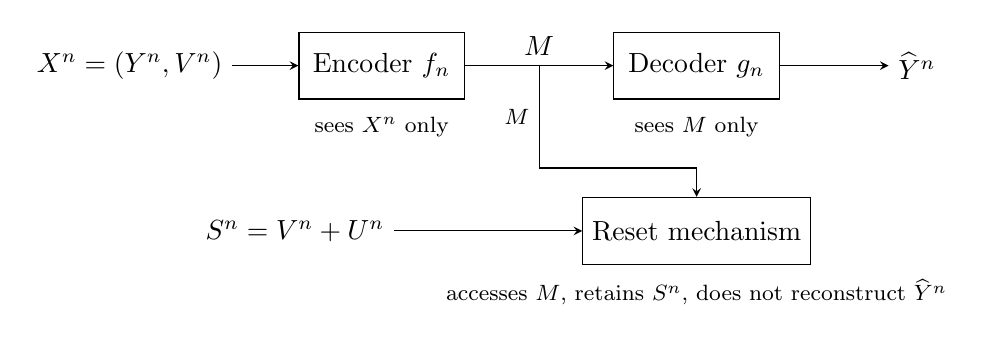
\begin{tikzpicture}[>=stealth,
  blk/.style={draw,rectangle,minimum height=0.85cm,minimum width=2.1cm},
  lbl/.style={font=\footnotesize}]
\node (x) at (-0.5,0) {$X^n=(Y^n,V^n)$};
\node[blk] (enc) at (2.7,0) {Encoder $f_n$};
\node[blk] (dec) at (6.7,0) {Decoder $g_n$};
\node (xhat) at (9.5,0) {$\hY^n$};
\node[blk] (rst) at (6.7,-2.1) {Reset mechanism};
\node (s) at (1.6,-2.1) {$S^n=V^n+U^n$};
\draw[->] (x) -- (enc);
\draw[->] (enc) -- node[above] {$M$} (dec);
\draw[->] (dec) -- (xhat);
\draw[->] (s) -- (rst);
\draw[->] (4.7,0) -- (4.7,-1.3) node[midway,left,lbl] {$M$} -| (rst.north);
\node[lbl] at (2.7,-0.78) {sees $X^n$ only};
\node[lbl] at (6.7,-0.78) {sees $M$ only};
\node[lbl] at (6.7,-2.88) {accesses $M$, retains $S^n$, does not
reconstruct $\hY^n$};
\end{tikzpicture}
\caption{The system. The encoder observes the source $X^n$ alone and stores
the description $M$ at rate $R_n$; the decoder reconstructs from $M$ alone;
the third party (the reset mechanism) retains the side information
$S^n$ and accesses the stored index $M$ in order to erase it; it never
reconstructs. The figure shows the Gaussian
instantiation, where the encoder observes $T=(Y,V)$, $S=V+U$ with $U$
independent of $T$, and
the reproduction is $\hY^n$, an estimate of $Y^n$ alone; the general
discrete theorem reproduces the full letter.}
\label{fig:system}
\end{figure}

A distortion measure is a bounded function
\begin{equation}
 d:\cX\times\widehat{\cX}\longrightarrow[0,d_{\max}].
\end{equation}
An $(n,\mathcal M_n)$ observation code consists of an encoder and decoder
\begin{equation}
 f_n:\cX^n\to\mathcal M_n,
 \qquad
 g_n:\mathcal M_n\to\widehat{\cX}^{n}.
\end{equation}
We write $M=f_n(X^n)$ and $\hXn=g_n(M)$. Randomized encoders do not improve
the region below, but allowing them in the converse is harmless.

The three operational quantities are
\begin{align}
 R_n&=\frac{1}{n}\log |\mathcal M_n|,\label{eq:rate-def}\\
 D_n&=\frac{1}{n}\sum_{i=1}^{n}\E\,d(X_i,\hX_i),\label{eq:dist-def}\\
 L_n&=\frac{1}{n}H(M\mid S^n).\label{eq:work-def}
\end{align}
The dimensionless quantity $L_n$ is the residual description content: the
uncertainty about the stored index that remains given the retained side
information. We call it the \emph{conditional content} of the memory relative
to the retained side information; the thermodynamic reading of
Remark~\ref{rem:thermo}, after the coding theorem, is the reason for
pricing it. Every statement and proof of the paper treats $L_n$ as
the coding quantity \eqref{eq:work-def}, in bits per source symbol.

\begin{definition}[Achievability]\label{def:achievability}
A triple $(R,L,D)$ is achievable if there is a sequence of observation codes
such that
\begin{equation}
 \limsup_{n\to\infty}R_n\le R,\qquad
 \limsup_{n\to\infty}L_n\le L,\qquad
 \limsup_{n\to\infty}D_n\le D.
\end{equation}
The closure of the achievable set at distortion $D$ is denoted $\RW(D)$.
\end{definition}

For a test channel $p(\hat x\mid x)$, the Markov chain $\hX-X-S$ holds
because side information is unavailable when the observation is formed.
Define
\begin{equation}
 \mathcal T(D)
 =\left\{p(\hat x\mid x):\E d(X,\hX)\le D\right\}.
\end{equation}
The two single-letter functions of the paper are the classical
rate--distortion function and the content endpoint,
\begin{equation}
 R_{\min}(D)=\min_{p(\hat x\mid x)\in\mathcal T(D)}I(X;\hX),
 \qquad
 L(D)=\min_{p(\hat x\mid x)\in\mathcal T(D)}I(X;\hX\mid S).
 \label{eq:work-endpoint}
\end{equation}
Both minima exist by compactness of $\mathcal T(D)$ and continuity of the
two coordinates. The coding theorem below gives both functions their
operational meaning. The following box fixes the two notational scopes of
the paper.

\begin{definition}[Problem statement: discrete and Gaussian scopes]\label{def:problem}
\emph{General letters}, used for the discrete theorem of this section:
source $(X,S)\sim p_{XS}$, i.i.d.\ copies $(X^n,S^n)$, test channel
$p(\hat x\mid x)$ with the Markov chain $\hX-X-S$, constraint set
$\mathcal T(D)$, and the two functions of \eqref{eq:work-endpoint}.
\emph{Gaussian letters}, used from Section~\ref{sec:pair} on: the source
letter is the jointly Gaussian pair $T=(Y,V)$ with
$\operatorname{Var}Y=\operatorname{Var}V=1$ and $\E[YV]=\rho$; the context
copy is generated as $S=V+U$ with $U\sim\mathcal N(0,\tau^2)$ independent
of everything else; the test channel is $p(\hat y\mid t)$, the reproduction
$\hY$ does not see $S$, and the Markov chain is $\hY-T-S$; the constraint
is $\E(Y-\hY)^2\le D$; and
\[
R_{\min}(D)=\min I(T;\hY),
\qquad
L(D)=\min I(T;\hY\mid S),
\]
both minima over test channels meeting the constraint.
\end{definition}

\begin{lemma}[Convexity in the test channel]\label{lem:convexity}
For fixed $p_{XS}$, both coordinates $I(X;\hX)$ and $I(X;\hX\mid S)$ are
convex functions of the test channel $q(\hat x\mid x)$.
\end{lemma}

\begin{proof}
Convexity of $I(X;\hX)$ in the channel at fixed input is classical. For the
conditional coordinate, the Markov chain $\hX-X-S$ gives
$p(\hat x\mid x,s)=q(\hat x\mid x)$, so
\begin{equation}
 I(X;\hX\mid S)=\sum_s p(s)\,I_{p(x\mid s)}(q),
 \label{eq:per-s-decomposition}
\end{equation}
a nonnegative combination of mutual informations, each with fixed input
distribution $p(x\mid s)$ and the common channel $q$; each term is convex in
$q$, hence so is the sum. We note that the decomposition
$I(X;\hX\mid S)=I(X;\hX)-I(S;\hX)$ does \emph{not} yield this conclusion:
$I(S;\hX)$ is itself convex in $q$ (the induced channel
$p(\hat x\mid s)=\sum_x p(x\mid s)q(\hat x\mid x)$ is linear in $q$), so the
difference is a priori indefinite.
\end{proof}

\begin{lemma}[Closure and right-continuity of the single-letter region]
\label{lem:rightcont}
For a finite-alphabet source $(X,S)$ and bounded distortion $d$, define
\[
\mathcal R(D):=\bigcup_{q\in\mathcal T(D)}
\bigl\{(R,L):R\ge I_q(X;\hX),\ L\ge I_q(X;\hX\mid S)\bigr\}.
\]
Then $\mathcal R(D)$ is closed and nondecreasing in $D$, and it is
right-continuous:
\[
\mathcal R(D)=\bigcap_{D'>D}\mathcal R(D').
\]
Equivalently, if $(R_j,L_j)\in\mathcal R(D_j)$ with
$(R_j,L_j)\to(R,L)$ and $\limsup_jD_j\le D$, then
$(R,L)\in\mathcal R(D)$.
\end{lemma}

\begin{proof}
Monotonicity is the nesting of the constraint sets $\mathcal T(D)$. For
the sequential form, pick $q_j\in\mathcal T(D_j)$ with
$R_j\ge I_{q_j}(X;\hX)$ and $L_j\ge I_{q_j}(X;\hX\mid S)$. The channels
live in the compact simplex of conditional distributions, so a
subsequence converges to some $q$; the distortion $\E_q\,d(X,\hX)$ is
continuous in the channel, so
$\E_q\,d=\lim_j\E_{q_j}d\le\limsup_jD_j\le D$ and $q\in\mathcal T(D)$.
Both mutual-information coordinates are continuous in the channel on
finite alphabets, so $I_q(X;\hX)=\lim_jI_{q_j}(X;\hX)\le R$ and
likewise $I_q(X;\hX\mid S)\le L$: the limit $(R,L)$ lies in $q$'s
quadrant, hence in $\mathcal R(D)$. Closedness is the sequential form
with $D_j\equiv D$. For right-continuity, the inclusion
$\mathcal R(D)\subseteq\bigcap_{D'>D}\mathcal R(D')$ is monotonicity,
and conversely a point of the intersection is a constant sequence with
$(R_j,L_j)\equiv(R,L)\in\mathcal R(D_j')$ along any $D_j'\downarrow D$,
so it lies in $\mathcal R(D)$ by the sequential form.
\end{proof}

\paragraph*{Architecture of the coding theorem}
The proof of Theorem~\ref{thm:main-region} below has six steps, and one
possible confusion is worth preempting at the outset: the reconstruction
decoder never sees $S^n$; the binning of Wyner--Ziv type appears only
inside an accounting argument. (i) The description rate comes from
ordinary covering: a rate--distortion codebook whose index $M$ the
decoder alone uses. (ii) Reconstruction is from the full index $M$.
(iii) A \emph{virtual} bin index $B=b(M)$ is introduced for
conditional-entropy accounting only; no party transmits or stores $B$.
(iv) A Fano bound controls the residual uncertainty about $M$ at a
\emph{hypothetical} decoder holding $(B,S^n)$; this hypothetical decoder
is a proof device, not a change of the model. (v) An expurgation step
selects one deterministic code satisfying the covering and the
accounting requirements simultaneously. (vi) The Gaussian source is
treated in Appendix~\ref{app:gaussian}, whose achievability invokes the
finite-alphabet theorem below on a quantized surrogate; the closed
forms of Sections~\ref{sec:pair}--\ref{sec:binary} are single-letter
evaluations that do not depend on it.

\begin{theorem}[Rate--content--distortion region]\label{thm:main-region}
For a discrete memoryless source $(X,S)$ and bounded distortion $d$,
\begin{equation}
\boxed{
 \RW(D)
 =\bigcup_{p(\hat x\mid x)\in\mathcal T(D)}
 \left\{(R,L):
 R\ge I(X;\hX),\
 L\ge I(X;\hX\mid S)
 \right\}.}
 \label{eq:main-region}
\end{equation}
By Lemma~\ref{lem:convexity} both coordinates are convex in the common
test channel, so the union is already convex, and it is closed and
right-continuous in the distortion level (Lemma~\ref{lem:rightcont});
consequently no time sharing is required, and every boundary point is
attained by a single test channel.
\end{theorem}

\begin{proof}
We first prove the converse. Let a code produce $M$ and $\hXn$. Since $\hXn$
is a function of $M$,
\begin{align}
 \log|\mathcal M_n|
 &\ge H(M)\ge I(X^n;M)\ge I(X^n;\hXn)\nonumber\\
 &\ge \sum_{i=1}^{n}I(X_i;\hX_i),
 \label{eq:rate-conv}
\end{align}
where the last step follows from memorylessness and conditioning reducing
entropy (Appendix~\ref{app:converse}). Likewise,
\begin{align}
 H(M\mid S^n)
 &\ge I(X^n;M\mid S^n)
 \ge I(X^n;\hXn\mid S^n)\nonumber\\
 &\ge \sum_{i=1}^{n}I(X_i;\hX_i\mid S_i).
 \label{eq:work-conv}
\end{align}
Each induced per-letter channel $p(\hat x_i\mid x_i)$ satisfies the Markov
constraint $\hX_i-X_i-S_i$: $\hX_i$ is a function of $(X_i,X_{\ne i})$ and
$S_i$ is independent of $X_{\ne i}$ given $X_i$ for i.i.d. pairs. Let
$\bar q(\hat x\mid x)=\frac1n\sum_{i=1}^{n}p(\hX_i=\hat x\mid X_i=x)$ be
the mixture channel; the constraint survives the mixture because
$p(s\mid x)$ is common across $i$. Its distortion is $D_n$, so
$\bar q\in\mathcal T(D_n)$, and by Lemma~\ref{lem:convexity},
\begin{equation*}
 R_n\ \ge\ \frac1n\sum_i I(X_i;\hX_i)\ \ge\ I_{\bar q}(X;\hX),
 \qquad
 L_n\ \ge\ \frac1n\sum_i I(X_i;\hX_i\mid S_i)\ \ge\ I_{\bar q}(X;\hX\mid S),
\end{equation*}
which places $(R_n,L_n)$ in the (already convex and closed) union of
\eqref{eq:main-region} at distortion $D_n$. The right side of
\eqref{eq:main-region} is the set $\mathcal R(D_n)$ of
Lemma~\ref{lem:rightcont}, so, for an achievable triple with
$\limsup D_n\le D$, the sequential form of that lemma places every
limit point of $(R_n,L_n)$, and with it $(R,L)$, in the right side of
\eqref{eq:main-region} at $D$.

For achievability, fix $p(\hat x\mid x)\in\mathcal T(D)$ and $\epsilon>0$.
Generate a random codebook $\mathcal C$ of $2^{n(I(X;\hX)+2\epsilon)}$
independent $\hat x^n$ codewords drawn from the $\hX$-marginal, and,
independently, a random binning $b$ assigning each codeword index
uniformly to one of $2^{n(I(X;\hX\mid S)+3\epsilon)}$ bins. The covering
encoder selects a codeword jointly (strongly) typical with $x^n$,
declaring failure otherwise, and stores its index $M$; the decoder
reconstructs the codeword from $M$ alone. Two failure events. First,
$E_{\mathrm{cov}}$: no jointly typical codeword exists;
$\Pr(E_{\mathrm{cov}})\to0$, averaged over $(X^n,\mathcal C)$, by the
covering lemma, and on $E_{\mathrm{cov}}^{\mathrm c}$ the distortion is
at most $D+\epsilon$ by typicality. Second, $E_{\mathrm{bin}}$: the
side-information proof device fails. Because $\hX-X-S$,
\begin{equation}
 I(X;\hX\mid S)=I(X;\hX)-I(S;\hX),
\end{equation}
so each bin holds $2^{n(I(S;\hX)-\epsilon)}$ codewords on average, a
per-bin codeword rate $\epsilon$ below the packing threshold $I(S;\hX)$,
and the Wyner--Ziv packing argument \cite{wynerziv1976} (the Markov lemma for
the typicality of the selected codeword with $S^n$, and the packing
bound for wrong codewords in the bin) gives a decoder that recovers $M$
from $(B,S^n)$, $B=b(M)$, with
$\Pr(E_{\mathrm{bin}})\to0$ averaged over $(X^n,S^n,\mathcal C,b)$.
This decoder is a proof device; the actual decoder of the code still
receives no side information.

\emph{Selection of one deterministic code.} Let
$\epsilon_n:=\E_{\mathcal C,b}\bigl[\Pr(E_{\mathrm{cov}}\mid\mathcal C)
+\Pr(E_{\mathrm{bin}}\mid\mathcal C,b)\bigr]\to0$. By Markov's
inequality there is a deterministic pair $(\mathcal C,b)$ with
$\Pr(E_{\mathrm{cov}})+\Pr(E_{\mathrm{bin}})\le2\epsilon_n$. Fix it.
Its distortion satisfies
$D_n\le D+\epsilon+2\epsilon_n d_{\max}$, and by Fano's inequality
applied to the proof device on this fixed code,
$H(M\mid B,S^n)\le1+2\epsilon_n\log|\mathcal M_n|
=1+2\epsilon_n\,n\bigl(I(X;\hX)+2\epsilon\bigr)$, so
\begin{align}
 H(M\mid S^n)
 &\le H(B)+H(M\mid B,S^n)\nonumber\\
 &\le n\bigl(I(X;\hX\mid S)+3\epsilon\bigr)
 +1+2\epsilon_n\,n\bigl(I(X;\hX)+2\epsilon\bigr)
 \;=\;n\bigl(I(X;\hX\mid S)+3\epsilon+o(1)\bigr).
 \label{eq:entropy-ach}
\end{align}
The selected deterministic code thus satisfies the distortion and the
conditional-entropy requirements simultaneously: the stored index has
ordinary description rate $I(X;\hX)+2\epsilon$, distortion at most
$D+\epsilon+o(1)$, and conditional content at most
$I(X;\hX\mid S)+3\epsilon+o(1)$. Letting $\epsilon\downarrow0$ along a
diagonal sequence of blocklengths exhibits the corner
$\bigl(I(X;\hX),I(X;\hX\mid S)\bigr)$ at distortion $D$; since the
union in \eqref{eq:main-region} is already convex and closed
(Lemmas~\ref{lem:convexity} and~\ref{lem:rightcont}), this exhibits
the entire region.
\end{proof}

The binning step in the proof has a simple interpretation. The full codeword
index is required by the decoder. Given the side information, the codeword
is identified up to a residual set of asymptotic size $2^{nI(X;\hX\mid S)}$; only
that residual uncertainty remains in the stored index. The step has also
been verified numerically at finite blocklength
(Appendix~\ref{app:numver}).

\begin{remark}[Thermodynamic reading]\label{rem:thermo}
This remark states the paper's only physical claim; everywhere else
$L_n$ and $L(D)$ are the coding quantities \eqref{eq:work-def} and
\eqref{eq:work-endpoint}. The reset model is that of stochastic
thermodynamics with side information: the third party holds the record
$M$ and the classical side information $S^n$, which is read without
disturbance and remains unchanged; it knows the joint law of $(M,S^n)$
induced by the code; it may drive $M$ by any protocol in contact with a
heat bath at temperature $T$, conditioned on $S^n$; the work supplied
may fluctuate from run to run and only its mean is counted; and only
$M$ is required to return to a standard state. Under these conditions
the generalized second law with correlations
\cite{sagawa2012,parrondo2015} bounds the average work of any process
that resets $M$ below by $\kb T\ln2\,H(M\mid S^n)$: Landauer's bound
\cite{landauer1961}, valid for arbitrary distributions
\cite{esposito2011}, with the entropy of the record reduced by its
mutual information with the retained side information. The bound is
attained by a quasi-static isothermal protocol conditioned on $S^n$, so
the minimal average work is exactly
\begin{equation}
 W_n^{\min}\;=\;\kb T\ln2\,H(M\mid S^n)\;=\;n\,\kb T\ln2\,L_n ,
 \label{eq:landauer-bound}
\end{equation}
with no error term and for every code. Hence, by
Theorem~\ref{thm:main-region}, and by Theorem~\ref{thm:gaussop} for the
Gaussian source, $L(D)$ is the least asymptotic average erasure work
per symbol, in units of $\kb T\ln2$, over codes meeting the distortion
constraint. This is the average-work setting. The single-shot,
deterministic-work setting of \cite{delrio2011,faist2015} prices the
same reset by smooth conditional entropies of the pair $(M,S^n)$, and
we make no claim in that setting. The scope of the claim:
\eqref{eq:landauer-bound} prices only the logically irreversible reset
of the volatile index $M$; it does not count the work of acquiring
$X^n$, driving a channel, correcting errors, or finishing in finite time
\cite{landauer1961,bennett1973}, and the codebook, wiring, and any
permanent lookup tables are part of the apparatus and are not erased in
each cycle. Physical units are restored by multiplying any content value
in bits per symbol by $\kb T\ln2$.
\end{remark}

The content-only endpoint of the region is the minimum conditional content, the
function $L(D)$ defined in \eqref{eq:work-endpoint}.
As an information quantity, $L(D)$ is Steinberg's common-reconstruction
rate--distortion function for side information $S$ \cite{steinberg2009}: the
reproduction must be determined without access to $S$. The operational roles
differ. In the common-reconstruction problem, $S$ is decoder side information
that must not corrupt reproducibility; here $S$ is held by a reset mechanism
that never serves the decoder. The remainder of the paper characterizes
$L(D)$, and the region around it, for the source of Section~\ref{sec:pair}.

\begin{remark}[The Gaussian pair specialization]\label{rem:specialization}
From Section~\ref{sec:pair} on, the source letter is the jointly Gaussian
pair $T=(Y,V)$ introduced there (the ambient source $X$ of that section
enters only through $T$, by Theorem~\ref{thm:pair}), and the distortion is
$d(x,\hat x)=(y-\hat y)^2$ on the $Y$ coordinate: the decoder is judged on
$Y$ alone, while the encoder observes the pair.
\end{remark}

\begin{remark}[Scope of the coding theorem]\label{rem:scope}
Theorem~\ref{thm:main-region} is stated and proved for finite alphabets and
bounded per-letter distortion. For the jointly Gaussian source of
Section~\ref{sec:pair} with quadratic distortion on the described
variable, the corresponding operational statement is
Theorem~\ref{thm:gaussop} in Appendix~\ref{app:gaussian}: the converse
is proved there in full, and the achievability by quantizing the conditioner, the source, and the
reproduction, invoking the finite-alphabet theorem, and passing to the
limit. The Gaussian closed forms of
Sections~\ref{sec:pair}--\ref{sec:vector} are evaluations of the
single-letter coordinates in \eqref{eq:main-region}, and their
operational meaning is inherited through Theorem~\ref{thm:gaussop}.
\end{remark}

Table~\ref{tab:notation} collects the notation used from here on.

\begin{table}[!t]
\caption{Notation.}
\label{tab:notation}
\centering
\footnotesize
\begin{tabular}{p{1.35in}p{4.55in}}
\hline
Symbol & Meaning\\
\hline
$T=(Y,V)$ & encoder-observed pair: described variable $Y$, context $V$
(normalized in Section~\ref{sec:pair}); $X$ is the ambient source, the
source letter of the discrete theorem\\
$S=V+U$ & the third party's copy; $U\sim\mathcal N(0,\tau^2)$
independent of $X$\\
$s=1+\tau^2$ & the context-noise parameter, the variance of $S$ after
normalization (scalar conditioner;
the vector-context section uses $\Sigma_U$, with conditioner covariance
$\Sigma_S=\Sigma_V+\Sigma_U$)\\
$\rho=\E[YV]$ & correlation of the described variable and the context\\
$D$ & distortion level, $\E(Y-\hY)^2\le D$\\
$M$, $R_n$, $L_n$ & stored index; rate $\tfrac1n\log|\mathcal M_n|$;
conditional content $\tfrac1n H(M\mid S^n)$\\
$R_{\min}(D)$, $L(D)$ & the two single-letter functions of
\eqref{eq:work-endpoint}\\
\hline
\multicolumn{2}{l}{\emph{Derived quantities}}\\
\hline
$(a,b)$, $\nu$ & regression coordinates of the test channel
$\hY=aY+bV+N$, and the noise variance $\nu=\operatorname{Var}N$
(Section~\ref{sec:function})\\
$Q_0$, $Q_1$ & unconditional and $S$-conditional signal parts of the
reproduction, $\operatorname{Var}(aY+bV)$ and
$\operatorname{Var}(aY+bV\mid S)$ (Section~\ref{sec:function})\\
$h(a,b)$ & noise-free distortion contribution
$\operatorname{Var}\bigl((1-a)Y-bV\bigr)$, so that
$\E(Y-\hY)^2=h+\nu$ \eqref{eq:distortion}\\
$\mu_c=(a\rho+b)/s$ & regression coefficient of the reproduction on
$S$ (proof of Theorem~\ref{thm:function})\\
$P(g)$, $g^\star$ & the quadratic \eqref{eq:Pg} and its larger root;
$L(D)=\tfrac12\log_2 g^\star$\\
$\alpha$; $\gamma_0$, $\gamma_1$ & frontier weight (rate versus
content); the two water levels $\nu/(Q_0+\nu)$ and $\nu/(Q_1+\nu)$
(Theorem~\ref{thm:region})\\
$\LRs(D)$, $\RLs(D)$ & conditional content of the rate-optimal channel;
rate of the content-optimal channel (Corollary~\ref{cor:misalign})\\
$\Lambda$, $c$, $y_0$ & whitened conditional covariance, regression
vector, and the unit vector with $Y=y_0^{\mathsf T}Z$
\eqref{eq:whitening} (Sections~\ref{sec:region}, \ref{sec:vector})\\
\hline
\end{tabular}
\end{table}

\section{Pair Sufficiency}
\label{sec:pair}

Let $X\sim\mathcal N(0,\Sigma_X)$ on $\R^d$, i.i.d. across source symbols.
The described variable is the linear functional $Y=w^{\mathsf T}X$; the third
party's copy is a second linear functional observed in noise,
$S=\gamma^{\mathsf T}X+U$. Normalize
$\operatorname{Var}(w^{\mathsf T}X)=1$ (rescaling $D$), write
$V=\gamma^{\mathsf T}X/\sigma_{\gamma}$, $\sigma_\gamma^2:=\gamma^{\mathsf T}\Sigma_X\gamma$,
the normalized context, with
$\rho:=\E[YV]$, $|\rho|<1$, and
rescale $S$ (invariantly for all mutual informations) to $S=V+U$,
$U\sim\mathcal N(0,\tau^2)$, $\tau^2>0$. Write $s=1+\tau^2$, the
context-noise parameter (a scalar, not to be confused with the random
variable $S$). Throughout,
$X$, $U$, and all channel randomness (including any resampling randomness
below) are \emph{mutually} independent. This joint form of the independence
assumption is essential: it is exactly what the $S$-kernel argument in
the next proof uses.

From here on the Gaussian scope of Definition~\ref{def:problem} is in
force: the ambient source is $X$, the pair is $T=(Y,V)$, the reproduction
is $\hY$, and once Theorem~\ref{thm:pair} below is proved, all
information quantities are written on $(T,\hY,S)$. Reproductions may be
taken scalar without loss of optimality: replacing
$\hX$ by $\hY:=w^{\mathsf T}\hX$ leaves the distortion unchanged and can
only decrease $I(X;\cdot\mid S)$ (conditional data processing), and
$\hY-X-S$ persists.

\paragraph*{Standing assumptions and degeneracies}
The Gaussian sections run under $0<D<1$, $|\rho|<1$, and $\tau^2>0$, and
every boundary is handled where it arises rather than excluded silently.
For $D\ge1$ the zero reproduction gives $R=L=0$, and $D=0$ is the
extended-real limit; both are recorded with the Gaussian operational
theorem (Appendix~\ref{app:gaussian}). The boundaries $\rho^2\in\{0,1\}$
are the anchor corners, the classical function at $\rho=0$ and
Steinberg's scalar formula as $\rho^2\to1$
(Corollary~\ref{cor:anchors}), and the frontier collapse at both is
computed in Corollary~\ref{cor:misalign}. The clean-context boundary
$\tau^2=0$ has its own branch wherever it matters:
Proposition~\ref{prop:marg} and the $\tau^2\to0$ anchor for the
function, and Remark~\ref{rem:cleanboundary} for the frontier; positivity
$\tau^2>0$ is exactly what makes $\Cov(T,S)\succ0$, the hypothesis of
the exhaustion lemma (Lemma~\ref{lem:gauss}). Degenerate covariances
reduce: $\Sigma_T\succ0$ is assumed, with linearly dependent components
dropped where noted, and singular channel residuals $\Sigma_N$ are
dispatched by Remark~\ref{rem:degenerate}. The closed form's root satisfies
$g^\star>1$ throughout $0<D<1$, $\tau^2>0$, by the bracketing
$P(1)=(D-1)\tau^2<0$ (Theorem~\ref{thm:function}).

\begin{theorem}[Pair sufficiency]\label{thm:pair}
In the problem
$L(D)=\min\{I(X;\hY\mid S):\hY-X-S,\ \E(Y-\hY)^2\le D\}$, it is without
loss of optimality to let the channel depend on $X$ only through
$T=(Y,V)$, and then $I(X;\hY\mid S)=I(T;\hY\mid S)$. Consequently $L(D)$
depends on $(\Sigma_X,w,\gamma,\tau^2)$, for the scalar linear functionals
$Y=w^{\mathsf T}X$ and $V=\gamma^{\mathsf T}X/\sigma_\gamma$ of a source of
arbitrary dimension $d$, only through $(\rho,\tau^2)$.
\end{theorem}
\begin{proof}
Given an admissible $p(\hat y\mid x)$, draw $\hY'$ from the conditional
law $p(\hat y\mid T=t)$ using fresh randomness. (a) $(T,\hY')\overset{d}=
(T,\hY)$, so the distortion (a functional of $(Y,\hY)$) is unchanged.
(b) $S=V+U$ with $U$ independent of $(X,\hY)$ and of $(X,\hY')$, so in
both joints the conditional density of $S$ given $(T,\hY)=(t,\hat y)$
is $p_U(\,\cdot-v)$: hence
$(T,\hY',S)\overset{d}=(T,\hY,S)$. (c) Given $T$, $\hY'$ is independent
of $(X,S)$, so $I(X;\hY'\mid S)=I(T;\hY'\mid S)+I(X;\hY'\mid T,S)
=I(T;\hY\mid S)\le I(X;\hY\mid S)$, the last step because $T$ is a
function of $X$. (d) $\hY'-X-S$ holds since $\hY'$ is a function of
$(X,\text{fresh noise})$ with the noise independent of $(X,U)$. The same
computation applied to a $T$-channel directly gives
$I(X;\hY\mid S)=I(T;\hY\mid S)$.
\end{proof}

This reduction is a distortion-preserving specialization of source-side
sufficiency for the information bottleneck. Armstrong \cite{armstrong2026}
establishes that replacing the source by a deterministic statistic
sufficient for the relevance variable leaves the bottleneck tradeoff
unchanged at every blocklength; Theorem~\ref{thm:pair} is the case in
which the source is $X$ and the statistic is $T=(Y,V)$, with the
addition that the
$T$-measurable mean-square distortion constraint is preserved, so the
reduction holds for the constrained functional and not only the
unconstrained bottleneck.

\section{The Function: Scalar Context}
\label{sec:function}

One further reduction identifies the class the closed form must beat.
\emph{(Marginalized class $=$ scalar corner.)} If the channel depends on $X$
only through $Y$ (that is, $\hY-Y-(X,S)$), then given $(Y,S)$, $\hY$ is
independent of $X$, so $I(X;\hY\mid S)=I(Y;\hY\mid S)$, and the class
optimum is exactly the scalar-corner value
$\tfrac12\log_2\bigl[(\sigma^2(1-\rho_{YS}^2)+\rho_{YS}^2D)/D\bigr]$ of the
pair $(Y,S)$, where $\sigma^2=\operatorname{Var}Y$ and $\rho_{YS}$ is the
correlation of that pair, $\rho_{YS}^2=\rho^2/s$ after the normalization
of Section~\ref{sec:pair} \cite{steinberg2009}; the
corner's converse applies to every $p(\hat y\mid y)$, discrete or not.

\begin{proposition}[Marginalization is strictly
suboptimal]\label{prop:marg}
Let $d=2$, $X\sim\mathcal N(0,I_2)$, $Y=X_1$, and $S=X_1+X_2$ (so
$\rho_{YS}^2=\tfrac12$ and $S$ is $X$-measurable). For $0<D<1$:
\begin{enumerate}
\item[(i)] the marginalized-class optimum is the scalar corner
$L_{\mathrm{marg}}(D)=\tfrac12\log_2\!\frac{1+D}{2D}$;
\item[(ii)] the vector problem has the exact value
\[
L_{\mathrm{vec}}(D)\;=\;\tfrac12\log_2^{+}\!\frac{1}{2D}
\;=\;R_{Y\mid S}(D),
\]
Gray's conditional rate--distortion function of $(Y,S)$ \cite{gray1973}
($\operatorname{Var}(Y\mid S)=\tfrac12$), attained by the linear channel
$\hY=(1-D)X_1+DX_2+N$, $N\sim\mathcal N(0,D(1-2D))$, for $D\le\tfrac12$,
and by $\hY=S/2$ (zero conditional content) for $D\ge\tfrac12$;
\item[(iii)] hence the strict gap
$L_{\mathrm{marg}}(D)-L_{\mathrm{vec}}(D)=\tfrac12\log_2(1+D)>0$ on
$(0,\tfrac12]$, and equals the full marginalized value on
$[\tfrac12,1)$ (where $L_{\mathrm{vec}}=0$; the absolute gap is decreasing
there, but it is all of $L_{\mathrm{marg}}$).
\end{enumerate}
\end{proposition}

\begin{proof}
(i) is the reduction above, evaluated at $\sigma^2=1$,
$\rho_{YS}^2=\tfrac12$.

(ii) \emph{Converse.} For any admissible $\hY$ (Markov $\hY-X-S$),
$I(X;\hY\mid S)\ge I(Y;\hY\mid S)$, and the induced conditional channel
$p(\hat y\mid y,s)$ is feasible for Gray's conditional problem at the same
distortion, so $I(Y;\hY\mid S)\ge R_{Y\mid S}(D)=\tfrac12\log_2^{+}
\bigl(\operatorname{Var}(Y\mid S)/D\bigr)=\tfrac12\log_2^{+}(1/(2D))$.
\emph{Achievability.} For $D\le\tfrac12$ take
$\hY=(1-D)X_1+DX_2+N$: distortion $D^2+D^2+D(1-2D)=D$;
$\operatorname{Var}(\hY)=1-D$, $\Cov(\hY,S)=1$,
$\operatorname{Var}(\hY\mid S)=1-D-\tfrac12=\tfrac12-D$, so
$I(X;\hY\mid S)=\tfrac12\log_2\frac{(1-2D)/2}{D(1-2D)}
=\tfrac12\log_2\frac1{2D}$. For $D\ge\tfrac12$, $\hY=S/2$ is a
deterministic function of $X$, has distortion
$\E\bigl((X_1-X_2)/2\bigr)^2=\tfrac12\le D$, and is constant given $S$, so
$I(X;\hY\mid S)=0$.

(iii) Subtract. The closed forms on both sides have been verified
numerically.
\end{proof}

The closed form occupies the rest of this section. By
Theorem~\ref{thm:pair} we restrict to $T$-channels, $T=(Y,V)$, with
scalar reproduction $\hY$. The working coordinates deserve a plain
statement before the machinery. Every jointly Gaussian test channel
takes the form $\hY=aY+bV+N$ with $N$ independent noise of variance
$\nu$, and every admissible channel, Gaussian or not, is measured through
the same three moments of its regression on $T$: the unconditional
signal part $Q_0=\operatorname{Var}(aY+bV)$, the $S$-conditional signal
part $Q_1=\operatorname{Var}(aY+bV\mid S)$, and the noise-free
distortion contribution $h=\operatorname{Var}\bigl((1-a)Y-bV\bigr)$, so
that $\E(Y-\hY)^2=h+\nu$. Everything from here through
Section~\ref{sec:vector} is expressed in $(a,b,\nu)$ and these moments;
Table~\ref{tab:notation} collects them. The converse rests on one
estimation-theoretic lemma. We state it for vector reproductions and
vector conditioners, in the generality that
Sections~\ref{sec:region} and~\ref{sec:vector} reuse.

\begin{lemma}[Gaussian exhaustion and the determinant identity]
\label{lem:gauss}
Let $(T,S)$ be jointly Gaussian and centered, $T\in\R^p$, $S\in\R^r$,
with $\Cov\bigl((T,S)\bigr)\succ0$. Let $\hat{\mathbf Y}\in\R^m$ be any
centered random vector with finite second moments, and define
\[
A:=\Cov(\hat{\mathbf Y},T)\,\Sigma_T^{-1}\in\R^{m\times p},\qquad
N':=\hat{\mathbf Y}-AT,\qquad
\Sigma_N:=\Cov(N')=\Cov(\hat{\mathbf Y})-A\Sigma_TA^{\mathsf T}.
\]
Assume $\Sigma_N\succ0$ and $\Cov(N',S)=0$. Then
\begin{equation}
I(T;\hat{\mathbf Y}\mid S)\;\ge\;\tfrac12\log_2
\frac{\det\Sigma_{T\mid S}}{\det\Sigma_e}
\;=\;\tfrac12\log_2
\frac{\det\bigl(A\Sigma_{T\mid S}A^{\mathsf T}+\Sigma_N\bigr)}
{\det\Sigma_N},
\label{eq:lem-cond}
\end{equation}
where $\Sigma_{T\mid S}=\Sigma_T-\Sigma_{TS}\Sigma_S^{-1}\Sigma_{ST}$
and $\Sigma_e$ is the error covariance of the best linear estimator of
$T$ from $(\hat{\mathbf Y},S)$. With $S$ deleted throughout, the
hypothesis $\Cov(N',S)=0$ becomes vacuous and the same argument gives
\begin{equation}
I(T;\hat{\mathbf Y})\;\ge\;\tfrac12\log_2
\frac{\det\bigl(A\Sigma_TA^{\mathsf T}+\Sigma_N\bigr)}{\det\Sigma_N}.
\label{eq:lem-rate}
\end{equation}
The jointly Gaussian channel $\hat{\mathbf Y}=AT+N$,
$N\sim\mathcal N(0,\Sigma_N)$ independent of $(T,S)$, realizes the same
second moments and attains both bounds with equality simultaneously.
\end{lemma}

\begin{proof}
\emph{Step 1: the max-entropy bound.} Write
$M:=\Cov\bigl((\hat{\mathbf Y},S)\bigr)$ and
$J:=\Cov\bigl(T,(\hat{\mathbf Y},S)\bigr)\in\R^{p\times(m+r)}$. First,
$M\succ0$: by the Schur-complement criterion on
\[
M=\begin{bmatrix}
\Cov(\hat{\mathbf Y})&\Cov(\hat{\mathbf Y},S)\\[2pt]
\Cov(S,\hat{\mathbf Y})&\Sigma_S
\end{bmatrix},
\]
positivity is equivalent to $\Sigma_S\succ0$ together with
$\Cov(\hat{\mathbf Y})-\Cov(\hat{\mathbf Y},S)\Sigma_S^{-1}
\Cov(S,\hat{\mathbf Y})\succ0$; the first holds because
$\Cov(T,S)\succ0$, and the second is evaluated in Step 2 to equal
$A\Sigma_{T\mid S}A^{\mathsf T}+\Sigma_N\succeq\Sigma_N\succ0$. The best
linear estimator of $T$ from $(\hat{\mathbf Y},S)$ is
$\widehat T=JM^{-1}(\hat{\mathbf Y};S)$, with error covariance
$\Sigma_e=\Sigma_T-JM^{-1}J^{\mathsf T}$. Since $(T,S)$ is jointly
Gaussian,
$h(T\mid S)=\tfrac12\log_2\bigl((2\pi e)^p\det\Sigma_{T\mid S}\bigr)$
exactly. For the other term, translation invariance of differential
entropy, the fact that conditioning reduces entropy, and the Gaussian maximum-entropy
bound at fixed covariance give
\[
h(T\mid\hat{\mathbf Y},S)
=h\bigl(T-\widehat T\;\big|\;\hat{\mathbf Y},S\bigr)
\;\le\;h\bigl(T-\widehat T\bigr)
\;\le\;\tfrac12\log_2\bigl((2\pi e)^p\det\Sigma_e\bigr)
\]
(with the usual convention that $h=-\infty$ for laws without a
density, in which case the bound is trivial).
Subtracting the two displays inside
$I(T;\hat{\mathbf Y}\mid S)=h(T\mid S)-h(T\mid\hat{\mathbf Y},S)$
yields the inequality in \eqref{eq:lem-cond}.

\emph{Step 2: the determinant identity.} Let
$K:=\Cov\bigl((T,S,\hat{\mathbf Y})\bigr)$. The residual $N'$ is
uncorrelated with $T$ by construction of the regression and with $S$ by
hypothesis, and the change of variables
$(T,S,\hat{\mathbf Y})\mapsto(T,S,N')$ is block lower triangular with
unit diagonal, hence determinant preserving:
\[
\det K=\det\Cov\bigl((T,S,N')\bigr)
=\det\begin{bmatrix}
\Sigma_T&\Sigma_{TS}&0\\
\Sigma_{ST}&\Sigma_S&0\\
0&0&\Sigma_N
\end{bmatrix}
=\det\Sigma_S\,\det\Sigma_{T\mid S}\,\det\Sigma_N,
\]
using in the last step the Schur factorization
$\det\Cov(T,S)=\det\Sigma_S\,\det\Sigma_{T\mid S}$. The same Schur
factorization applied to $K$ in the other block order gives
$\det K=\det M\,\det\Sigma_e$, and applied to $M$ itself gives
\[
\det M=\det\Sigma_S\cdot\det\Bigl(\Cov(\hat{\mathbf Y})
-\Cov(\hat{\mathbf Y},S)\Sigma_S^{-1}\Cov(S,\hat{\mathbf Y})\Bigr).
\]
It remains to evaluate the conditional block. From
$\hat{\mathbf Y}=AT+N'$ with $\Cov(N',T)=0$ and $\Cov(N',S)=0$,
$\Cov(\hat{\mathbf Y})=A\Sigma_TA^{\mathsf T}+\Sigma_N$ and
$\Cov(\hat{\mathbf Y},S)=A\Sigma_{TS}$, so
\[
\Cov(\hat{\mathbf Y})-\Cov(\hat{\mathbf Y},S)\Sigma_S^{-1}
\Cov(S,\hat{\mathbf Y})
=A\bigl(\Sigma_T-\Sigma_{TS}\Sigma_S^{-1}\Sigma_{ST}\bigr)A^{\mathsf T}
+\Sigma_N
=A\Sigma_{T\mid S}A^{\mathsf T}+\Sigma_N .
\]
Combining the three displays,
\[
\det\Sigma_e=\frac{\det K}{\det M}
=\frac{\det\Sigma_{T\mid S}\,\det\Sigma_N}
{\det\bigl(A\Sigma_{T\mid S}A^{\mathsf T}+\Sigma_N\bigr)},
\]
which is the identity in \eqref{eq:lem-cond}; in particular
$\Sigma_e\succ0$, so Step 1's bound is finite. Deleting $S$ (formally
$r=0$: $K=\Cov(T,\hat{\mathbf Y})$, $M=\Cov(\hat{\mathbf Y})$) gives
$\det\Sigma_{e0}=\det\Sigma_T\det\Sigma_N/
\det(A\Sigma_TA^{\mathsf T}+\Sigma_N)$ and hence \eqref{eq:lem-rate}.

\emph{Step 3: equality.} For the stated Gaussian channel the conditional
law of $T$ given $(\hat{\mathbf Y},S)$ is Gaussian with covariance
$\Sigma_e$ for every realization, so
$h(T\mid\hat{\mathbf Y},S)=\tfrac12\log_2\bigl((2\pi e)^p
\det\Sigma_e\bigr)$ and \eqref{eq:lem-cond} holds with equality;
likewise for \eqref{eq:lem-rate}. The channel's moments match those of
the given channel: $\Cov(AT+N,T)=A\Sigma_T$ and
$\Cov(AT+N)=A\Sigma_TA^{\mathsf T}+\Sigma_N$.
\end{proof}

\begin{remark}[Degenerate residuals]\label{rem:degenerate}
If $\Sigma_N$ is singular, some combination
$\eta^{\mathsf T}\hat{\mathbf Y}$ equals $\eta^{\mathsf T}AT$ almost
surely. If $\eta^{\mathsf T}A\ne0$ the reproduction reveals a noiseless linear
functional of the continuous $T$, so
$I(T;\hat{\mathbf Y}\mid S)=\infty$ and every bound below holds
trivially; if $\eta^{\mathsf T}A=0$ that combination of the reproduction is
zero and may be dropped, reducing $m$. All uses of
Lemma~\ref{lem:gauss} below may therefore assume $\Sigma_N\succ0$.
\end{remark}

\begin{theorem}[The closed form]\label{thm:function}
With $s=1+\tau^2$, the context-noise parameter of
Section~\ref{sec:pair}, for $0<D<1$,
\begin{equation}
L(D)=\tfrac12\log_2 g^\star,\qquad
g^\star=\frac{(D+s-\rho^2)+\sqrt{(D+s-\rho^2)^2-4Ds(1-\rho^2)}}{2Ds},
\label{eq:quadratic}
\end{equation}
the larger root of the quadratic
\begin{equation}
P(g)=Dsg^2-(D+s-\rho^2)g+(1-\rho^2).
\label{eq:Pg}
\end{equation}
Since $P(1)=(D-1)\tau^2<0$, exactly one root exceeds $1$, so $g^\star$
is well defined. The optimum is attained by the jointly Gaussian channel
\begin{equation}
\hY=aY+bV+N,\qquad
a=\frac{g^\star-1}{g^\star},\quad
b=\frac{(g^\star-1)\rho}{g^\star k},\quad
k=g^\star s-1,\quad
N\sim\mathcal N\Bigl(0,\;\frac{Q_1}{g^\star-1}\Bigr),
\label{eq:channel}
\end{equation}
where $Q_1=a^2+b^2+2ab\rho-(a\rho+b)^2/s$ is evaluated at these
$(a,b)$.
\end{theorem}

\begin{proof}
\emph{Moments.} By Theorem~\ref{thm:pair} and the scalar-reproduction
reduction of Section~\ref{sec:pair}, restrict to channels
$p(\hat y\mid t)$. Fix an admissible channel with
$\E(Y-\hY)^2\le D$. Centering $\hY$ leaves $I(T;\hY\mid S)$ unchanged
and can only decrease the distortion, so take $\E\hY=0$. Define the
regression coordinates
\[
\begin{pmatrix}a\\b\end{pmatrix}
:=\Sigma_T^{-1}\begin{pmatrix}\E[Y\hY]\\ \E[V\hY]\end{pmatrix},
\qquad
Q_0:=a^2+b^2+2ab\rho=\operatorname{Var}(aY+bV),
\qquad
\nu:=\operatorname{Var}\hY-Q_0,
\]
so that $\E[Y\hY]=a+b\rho$ and $\E[V\hY]=a\rho+b$; $\nu\ge0$ is the
residual variance of $\hY$ after linear regression on $T$. If $\nu=0$,
Remark~\ref{rem:degenerate} applies: either $(a,b)\ne(0,0)$ and
$I(T;\hY\mid S)=\infty$, or $(a,b)=(0,0)$ and $\hY=0$ with distortion
$1>D$. So take $\nu>0$.

\emph{The Markov moment identity.} The residual $N'=\hY-aY-bV$ is
uncorrelated with $T$ by construction. It is also uncorrelated with
$S=V+U$: it is uncorrelated with $V$, a coordinate of $T$, and
$\E[UN']=0$ because $U$ is independent of $(X,\hY)$ by the mutual
independence of $X$, $U$, and the channel randomness. Hence
$\Cov(N',S)=0$, which is the hypothesis of Lemma~\ref{lem:gauss}, and
which restates the moment identity $\E[S\hY]=\E[V\hY]$.

\emph{The converse bound, written out.} Here $p=2$, $m=1$, $r=1$,
$A=(a,b)$, $\Sigma_N=\nu$, and
\[
\Sigma_T=\begin{bmatrix}1&\rho\\ \rho&1\end{bmatrix},
\qquad
\Sigma_{TS}=\begin{bmatrix}\rho\\ 1\end{bmatrix},
\qquad
\Sigma_S=s,
\]
\[
\Sigma_{T\mid S}
=\Sigma_T-\frac1s\,\Sigma_{TS}\Sigma_{TS}^{\mathsf T}
=\begin{bmatrix}1-\rho^2/s&\rho\tau^2/s\\[2pt]
\rho\tau^2/s&\tau^2/s\end{bmatrix},
\qquad
\det\Sigma_{T\mid S}=\frac{\tau^2(1-\rho^2)}{s}>0 .
\]
The quadratic form in \eqref{eq:lem-cond} is
\[
A\Sigma_{T\mid S}A^{\mathsf T}
=Q_0-\frac{(a\rho+b)^2}{s}
=\operatorname{Var}(aY+bV\mid S)=:Q_1 ,
\]
and, explicitly, $M=\Cov\bigl((\hY,S)\bigr)=
\bigl[\begin{smallmatrix}Q_0+\nu&a\rho+b\\ a\rho+b&s\end{smallmatrix}\bigr]$
with $\det M=s(Q_0+\nu)-(a\rho+b)^2=s(Q_1+\nu)$, while
$\det\Cov\bigl((T,S,\hY)\bigr)=s\,\det\Sigma_{T\mid S}\cdot \nu$, so
$\det\Sigma_e=\nu\det\Sigma_{T\mid S}/(Q_1+\nu)$ and Lemma~\ref{lem:gauss}
reads
\begin{equation}
I(T;\hY\mid S)\;\ge\;
\tfrac12\log_2\frac{\det\Sigma_{T\mid S}}{\det\Sigma_e}
\;=\;\tfrac12\log_2\frac{Q_1+\nu}{\nu} .
\label{eq:scalar-detid}
\end{equation}
The distortion is a function of the same moments:
\begin{equation}
\E(Y-\hY)^2=1-2(a+b\rho)+Q_0+\nu=h(a,b)+\nu,
\qquad
h(a,b):=(1-a)^2-2(1-a)b\rho+b^2,
\label{eq:distortion}
\end{equation}
and $h(a,b)=\operatorname{Var}\bigl((1-a)Y-bV\bigr)\ge0$. Therefore
\begin{equation}
L(D)\;\ge\;
\inf\Bigl\{B(a,b,\nu):=\tfrac12\log_2\tfrac{Q_1+\nu}{\nu}
\;:\;h(a,b)+\nu\le D,\ \nu>0\Bigr\},
\label{eq:moment-program}
\end{equation}
and it suffices to evaluate the right side; achievability below
matches it.

\emph{Activity, coercivity, existence.} At fixed $(a,b)$ with $Q_1>0$,
$B$ is strictly decreasing in $\nu$
($\partial_\nu[\ln(Q_1+\nu)-\ln \nu]=(Q_1+\nu)^{-1}-\nu^{-1}<0$), so the infimum
is unchanged by imposing the active constraint $\nu=D-h(a,b)$. On the
feasible set, $(a,b)$ is confined to the compact set $\{h\le D\}$;
since $\Sigma_{T\mid S}\succ0$, the form
$Q_1=(a,b)\,\Sigma_{T\mid S}\,(a,b)^{\mathsf T}$ vanishes only at
$(a,b)=(0,0)$, where $h=1>D$, so by continuity $Q_1\ge q_0>0$ on the
feasible set. Hence $B\ge\tfrac12\log_2\bigl((q_0+\nu)/\nu\bigr)\to\infty$
as $\nu\to0$, the sublevel sets of the reduced objective
\[
\Phi(a,b):=\tfrac12\log_2\frac{Q_1(a,b)+\nu(a,b)}{\nu(a,b)},
\qquad \nu(a,b)=D-h(a,b),
\]
are compact, and the infimum in \eqref{eq:moment-program} is attained
at some $(a,b)$ with $h(a,b)<D$: an interior stationary point of
$\Phi$.

\emph{The stationarity system is linear in $(a,b)$ at fixed $g$.} At a
stationary point write $g:=(Q_1+\nu)/\nu$ and $\mu_c:=(a\rho+b)/s$; note
$g>1$ because $Q_1>0$. The partial derivatives of the three quadratics
are
\[
\partial_aQ_0=2(a+b\rho),\qquad
\partial_bQ_0=2(b+a\rho),\qquad
\partial_ah=\partial_aQ_0-2,\qquad
\partial_bh=\partial_bQ_0-2\rho,
\]
\[
\partial_aQ_1=\partial_aQ_0-2\rho\mu_c,\qquad
\partial_bQ_1=\partial_bQ_0-2\mu_c,
\]
hence the four gradient identities
\begin{equation}
\partial_a(Q_0-h)=2,\quad
\partial_b(Q_0-h)=2\rho,\quad
\partial_a(Q_1-h)=2(1-\rho\mu_c),\quad
\partial_b(Q_1-h)=2(\rho-\mu_c).
\label{eq:grad-ids}
\end{equation}
(Only the last two enter here; all four enter the weighted system of
Section~\ref{sec:region}.) With $\nu=D-h$, so
$\partial_xn=-\partial_xh$, stationarity of
$2\ln2\cdot\Phi=\ln(Q_1+\nu)-\ln \nu$ in $x\in\{a,b\}$ reads
\[
\frac{\partial_x(Q_1-h)}{Q_1+\nu}+\frac{\partial_xh}{\nu}=0,
\qquad\text{that is,}\qquad
\frac1g\,\partial_x(Q_1-h)+\partial_xh=0 .
\]
By \eqref{eq:grad-ids} and
$\partial_ah=2(a+b\rho-1)$, $\partial_bh=2(a\rho+b-\rho)$, the two
equations are
\begin{equation}
a+b\rho=1-\frac{1-\rho\mu_c}{g},
\qquad
a\rho+b=\rho-\frac{\rho-\mu_c}{g} .
\label{eq:foc}
\end{equation}
Substituting $\mu_c=(a\rho+b)/s$ makes \eqref{eq:foc} a $2\times2$
linear system in $(a,b)$ whose coefficients depend on $g$ alone, and it
solves in closed form. The second equation reads
$gs\mu_c-\mu_c=\rho(g-1)$, so with $k:=gs-1>0$,
\begin{equation}
\mu_c=\frac{\rho(g-1)}{k} .
\label{eq:mu}
\end{equation}
Subtracting $\rho$ times the first equation of \eqref{eq:foc} from the
second gives
$(a\rho+b)-\rho(a+b\rho)=b(1-\rho^2)$ on the left and
$\mu_c(1-\rho^2)/g$ on the right, so $b=\mu_c/g$; the first equation
then yields $a=1-(1-\rho\mu_c)/g-b\rho=1-1/g$. The stationary channel
coefficients at level $g$ are therefore
\begin{equation}
1-a=\frac1g,
\qquad
b=\frac{\mu_c}{g}=\frac{(g-1)\rho}{gk} .
\label{eq:ab}
\end{equation}

\emph{Reduction to the quadratic.} At the values \eqref{eq:ab},
$(1-a)Y-bV=(Y-\mu_cV)/g$, so
\begin{equation}
h=\frac{1-2\rho\mu_c+\mu_c^2}{g^2},
\label{eq:h-at-foc}
\end{equation}
and, writing $aY+bV=Y-(Y-\mu_cV)/g$ and using the definition
$a\rho+b=s\mu_c$,
\[
Q_0=1-\frac{2(1-\rho\mu_c)}{g}+h,
\qquad
Q_1=Q_0-\frac{(a\rho+b)^2}{s}
=1-\frac{2(1-\rho\mu_c)}{g}+h-s\mu_c^2 .
\]
The definition of $g$ and the active constraint combine to
$(g-1)(D-h)=Q_1$. Substituting the display for $Q_1$ and collecting
the $h$ terms ($h+(g-1)h=gh=(1-2\rho\mu_c+\mu_c^2)/g$ by
\eqref{eq:h-at-foc}), the terms in $\rho\mu_c$ cancel and
\begin{equation}
1+\frac{\mu_c^2-1}{g}-s\mu_c^2=(g-1)D .
\label{eq:pre-quadratic}
\end{equation}
Finally substitute \eqref{eq:mu}. Multiplying
\eqref{eq:pre-quadratic} by $gk^2$ and using
$k^2\mu_c^2=\rho^2(g-1)^2$,
\[
gk^2+\rho^2(g-1)^2-k^2-gs\rho^2(g-1)^2=g(g-1)Dk^2 .
\]
Since $1-gs=-k$, the second and fourth terms on the left combine to
$-\rho^2(g-1)^2k$, so the left side is
$(g-1)k\bigl[k-\rho^2(g-1)\bigr]$, and dividing by $(g-1)k>0$,
\[
k-\rho^2(g-1)=gDk
\quad\Longleftrightarrow\quad
Dsg^2-(D+s-\rho^2)g+(1-\rho^2)=0,
\]
that is, $P(g)=0$. Every interior stationary point of $\Phi$ therefore
sits at a root of $P$ exceeding $1$.

\emph{Root bracketing and uniqueness.}
$P(1)=Ds-(D+s-\rho^2)+(1-\rho^2)=(D-1)(s-1)=(D-1)\tau^2<0$ for $D<1$,
$\tau^2>0$. The leading coefficient $Ds$ is positive and
$P(0)=1-\rho^2>0$, so $P$ has two real roots, exactly one exceeding
$1$ (the other lies in $(0,1)$). Hence every stationary point has
$g=g^\star$, and by \eqref{eq:ab} the stationary $(a,b)$, and with it
$\nu=Q_1/(g^\star-1)$, is unique. The attained minimum of
\eqref{eq:moment-program} is $\tfrac12\log_2 g^\star$.

\emph{Achievability.} The channel \eqref{eq:channel} has exactly the
moments \eqref{eq:ab} with residual variance $\nu=Q_1/(g^\star-1)$. Its
distortion is $h+\nu$, and $(g^\star-1)\nu=Q_1$ together with
$P(g^\star)=0$ is, by the chain of equivalences above run backward,
the statement $h+\nu=D$. The channel is jointly Gaussian with $(T,S)$,
so the equality clause of Lemma~\ref{lem:gauss} gives
\[
I(T;\hY\mid S)=\tfrac12\log_2\frac{Q_1+\nu}{\nu}=\tfrac12\log_2 g^\star .
\]
Hence $L(D)=\tfrac12\log_2 g^\star$.
\end{proof}

\begin{corollary}[The three classical corners]\label{cor:anchors}
(i) At $\rho=0$, $P(g)=(Dg-1)(sg-1)$ and $g^\star=1/D$:
$L(D)=\tfrac12\log_2(1/D)$ is the classical rate--distortion function,
attained with $b=0$ by the classical reverse test channel.
(ii) As $\tau^2\to0$,
$L(D)\to\tfrac12\log_2^{+}\bigl((1-\rho^2)/D\bigr)$, Gray's
conditional rate--distortion function of the pair $(Y,V)$
\cite{gray1973}, matching Proposition~\ref{prop:marg}.
(iii) As $\rho^2\to1$,
$L(D)\to\tfrac12\log_2\bigl[(D+\tau^2)/(D(1+\tau^2))\bigr]$,
Steinberg's scalar Gaussian formula at the induced correlation
$\rho_{YS}^2=1/s$ \cite{steinberg2009}.
\end{corollary}

\begin{proof}
(i) $(Dg-1)(sg-1)=Dsg^2-(D+s)g+1=P(g)\big|_{\rho=0}$. The roots are
$1/D>1$ and $1/s<1$, so $g^\star=1/D$. At this root \eqref{eq:channel}
gives $b=0$, $a=1-D$, $Q_1=(1-D)^2$, and
$\operatorname{Var}N=(1-D)^2/(1/D-1)=D(1-D)$: the classical reverse
channel.

(ii) At $s=1$,
$P(g)=Dg^2-(D+1-\rho^2)g+(1-\rho^2)=(g-1)\bigl(Dg-(1-\rho^2)\bigr)$,
with discriminant $\bigl(D-(1-\rho^2)\bigr)^2$, so the larger root at
$s=1$ is exactly $\max\{1,(1-\rho^2)/D\}$; the roots of $P$ are
continuous in $s$, and the limit follows. For $D<1-\rho^2$ the value
is $\tfrac12\log_2\bigl(\operatorname{Var}(Y\mid V)/D\bigr)$ with
$\operatorname{Var}(Y\mid V)=1-\rho^2$, Gray's conditional function;
for $D\ge1-\rho^2$ it is $0$.

(iii) At $\rho^2=1$ the constant term of $P$ vanishes:
$P(g)=g\bigl(Dsg-(D+\tau^2)\bigr)$, with roots $0$ and
$(D+\tau^2)/(Ds)$; the latter exceeds $1$ because
$(D+\tau^2)-Ds=\tau^2(1-D)>0$. By root continuity
$g^\star\to(D+\tau^2)/(Ds)$ as $\rho^2\to1$. Steinberg's scalar
function at unit source variance and side-information correlation
$\rho_{YS}^2$ is
$\tfrac12\log_2\bigl[(1-\rho_{YS}^2+\rho_{YS}^2D)/D\bigr]$
\cite{steinberg2009}; at $\rho_{YS}^2=\rho^2/s\to1/s$
this is $\tfrac12\log_2\bigl[(\tau^2+D)/(sD)\bigr]$, the same value.
\end{proof}

\begin{remark}[Convergence rates at the anchors]\label{rem:anchorrates}
Each anchor of Corollary~\ref{cor:anchors} is approached at a linear
rate, with an explicit first-order coefficient. In every case the
anchor value is a simple root of $P$ ($P'(g^\star)\ne0$, evaluated
below), so the root is differentiable in the perturbing parameter
$\epsilon$ with $dg^\star/d\epsilon=-P_\epsilon/P'(g^\star)$, and
$L=\tfrac12\log_2 g^\star$ converts the derivative to the gap
coefficient; the three evaluations are verified symbolically and
numerically (Appendix~\ref{app:numver}). All values are in bits; the
factor $\ln2$ converts the natural-log derivative to base two.
(i) As $\rho^2\to0$ at fixed $(\tau^2,D)$, with $P'(1/D)=s-D>0$,
\[
L(D)-\tfrac12\log_2\frac1D
=-\frac{1-D}{2\ln2\,(s-D)}\,\rho^2+O(\rho^4):
\]
the gap to the classical rate--distortion function closes linearly in
$\rho^2$ with coefficient $-(1-D)/\bigl(2\ln2\,(s-D)\bigr)$, from
below (even a weakly correlated context lowers the conditional
content; $L(D)\le R_{\min}(D)$ always, with equality at $\rho=0$).
(ii) As $\tau^2\to0$ at fixed $(\rho^2,D)$, $D<1-\rho^2$, with
$P'\bigl((1-\rho^2)/D\bigr)=1-\rho^2-D>0$ at $s=1$,
\[
L(D)-\tfrac12\log_2\frac{1-\rho^2}{D}
=\frac{\rho^2}{2\ln2\,(1-\rho^2-D)}\,\tau^2+O(\tau^4):
\]
the gap to Gray's conditional function closes linearly in $\tau^2$,
from above, with coefficient $\rho^2/\bigl(2\ln2\,(1-\rho^2-D)\bigr)$.
The coefficient diverges as $D\uparrow1-\rho^2$, where the two roots of
$P$ collide at $g=1$ and the linear rate fails; on the far branch
$D>1-\rho^2$, where Gray's value is zero, the gap is $L(D)$ itself and
closes linearly with coefficient
$(1-D)/\bigl(2\ln2\,(D-(1-\rho^2))\bigr)$.
(iii) As $\rho^2\to1$ at fixed $(\tau^2,D)$, with
$P'\bigl((D+\tau^2)/(Ds)\bigr)=D+\tau^2>0$,
\[
L(D)-\tfrac12\log_2\frac{D+\tau^2}{Ds}
=\frac{\tau^2(1-D)}{2\ln2\,(D+\tau^2)^2}\,(1-\rho^2)
+O\bigl((1-\rho^2)^2\bigr):
\]
the gap to Steinberg's scalar formula closes linearly in $1-\rho^2$,
from above, with coefficient
$\tau^2(1-D)/\bigl(2\ln2\,(D+\tau^2)^2\bigr)$.
\end{remark}

\section{The Rate--Content Region and Misalignment}
\label{sec:region}

The content-only endpoint of Theorem~\ref{thm:function} does not come for
free in rate. This section characterizes the full tradeoff between the
two coordinates of \eqref{eq:main-region} for the Gaussian pair source.
Throughout, $\rho^2\in(0,1)$, $\tau^2>0$, $0<D<1$, and $h$, $Q_0$,
$Q_1$, $\mu_c$ are as in the proof of Theorem~\ref{thm:function}. In
the frontier system below, $\alpha\in[0,1]$ weights rate against
conditional content, and $\gamma_0=\nu/(Q_0+\nu)$ and $\gamma_1=\nu/(Q_1+\nu)$
are the two water levels the stationarity system balances: the
frontier point at weight $\alpha$ is
$\bigl(\tfrac12\log_2(1/\gamma_0),\,\tfrac12\log_2(1/\gamma_1)\bigr)$.
The name is used in a narrow sense: $\gamma_0$ and $\gamma_1$ are
called water levels because they play the inverse
signal-plus-noise roles in the two mutual-information coordinates;
unlike classical parallel-channel water-filling, in which independent
subchannels receive separate allocations, the two levels here are
coupled through one reproduction and one distortion constraint.

\begin{theorem}[The rate--content region]\label{thm:region}
The closure of the single-letter rate--content pairs
$\bigl(I(T;\hY),\,I(T;\hY\mid S)\bigr)$ over admissible test channels
at distortion $D$, which Theorem~\ref{thm:gaussop} identifies with the
operational region $\RW(D)$, is
the closed convex set whose Pareto frontier is traced by
$\alpha\in[0,1]$ as follows. Let
$(a,b,\nu,\gamma_0,\gamma_1)$, with $\nu>0$ and
$\gamma_0,\gamma_1\in(0,1)$, solve the stationarity system
\begin{equation}
a=1-\alpha\gamma_0-(1-\alpha)\gamma_1,
\qquad
\mu_c=\frac{a\rho}{s-(1-\alpha)\gamma_1},
\qquad
b=(1-\alpha)\gamma_1\mu_c,
\label{eq:twolevel-1}
\end{equation}
\begin{equation}
\nu=D-h(a,b),
\qquad
\gamma_0=\frac{\nu}{Q_0+\nu},
\qquad
\gamma_1=\frac{\nu}{Q_1+\nu}.
\label{eq:twolevel-2}
\end{equation}
The solution exists and is unique at every $\alpha$
(Proposition~\ref{prop:uniq} below; at $\alpha=0$ uniqueness also follows
from Theorem~\ref{thm:function}), and the frontier point is
\[
\bigl(R(\alpha),L(\alpha)\bigr)
=\Bigl(\tfrac12\log_2\frac1{\gamma_0},\
\tfrac12\log_2\frac1{\gamma_1}\Bigr),
\]
achieved by $\hY=aY+bV+N$, $N\sim\mathcal N(0,\nu)$. Endpoints:
$\alpha=1$ recovers the classical reverse channel ($b=0$, $a=1-D$,
$\gamma_0=D$, $R=\tfrac12\log_2(1/D)$); $\alpha=0$ recovers the channel
and value of Theorem~\ref{thm:function} ($\gamma_1=1/g^\star$).
\end{theorem}

\begin{proof}
\emph{Convexity and scalarization.} Both coordinates are convex in the
test channel: Lemma~\ref{lem:convexity} and the per-$s$ decomposition
\eqref{eq:per-s-decomposition} apply verbatim with the sum over $s$
replaced by an integral against the law of $S$, the conditional laws
$p(t\mid s)$ being furnished by disintegration through a regular
conditional probability ($S$ takes values in a standard Borel space).
The achievable set of pairs at distortion $D$ is therefore convex,
closed, and upward closed in each coordinate, so every point of its
Pareto frontier minimizes one of the weighted objectives
\[
J_\alpha:=\alpha\,I(T;\hY)+(1-\alpha)\,I(T;\hY\mid S),
\qquad\alpha\in[0,1],
\]
over admissible channels, by the supporting-hyperplane argument. At
the interior weights each $J_\alpha$-minimizer is a frontier point;
at the endpoint weights $\alpha\in\{0,1\}$ this a priori fixes only
one coordinate of the minimizer, and the value of the other
coordinate is pinned by the uniqueness of the minimizing moments
(Proposition~\ref{prop:uniq} below; the argument is run in detail in
the proof of Corollary~\ref{cor:misalign} at the end of this section).

\emph{The two determinant identities.} Fix an admissible channel,
centered without loss, with regression coordinates $(a,b,\nu)$, $\nu>0$,
as in the proof of Theorem~\ref{thm:function}; the Markov moment
identity $\Cov(N',S)=0$ holds as there. Lemma~\ref{lem:gauss} applies
twice to the same three moments, once with the conditioner $S$ and once
with $S$ deleted:
\begin{equation}
I(T;\hY)\ \ge\
\tfrac12\log_2\frac{\det\Sigma_T}{\det\Sigma_{e0}}
=\tfrac12\log_2\frac{Q_0+\nu}{\nu},
\qquad
I(T;\hY\mid S)\ \ge\
\tfrac12\log_2\frac{\det\Sigma_{T\mid S}}{\det\Sigma_{e}}
=\tfrac12\log_2\frac{Q_1+\nu}{\nu},
\label{eq:two-detids}
\end{equation}
where $\Sigma_{e0}$ is the error covariance of the best linear
estimate of $T$ from $\hY$ alone. The conditional identity is written
out in the proof of Theorem~\ref{thm:function}. The rate identity, in
full: with $\hat c:=\E[T\hY]=\Sigma_T(a,b)^{\mathsf T}$ and
$\operatorname{Var}\hY=Q_0+\nu$,
\[
\Sigma_{e0}=\Sigma_T-\frac{\hat c\,\hat c^{\mathsf T}}{Q_0+\nu},
\qquad
\det\Sigma_{e0}
=\det\Sigma_T\,
\Bigl(1-\frac{\hat c^{\mathsf T}\Sigma_T^{-1}\hat c}{Q_0+\nu}\Bigr)
=\det\Sigma_T\,\frac{\nu}{Q_0+\nu},
\]
by the rank-one determinant identity
$\det(\Sigma-\hat c\hat c^{\mathsf T}/v)
=\det\Sigma\,(1-\hat c^{\mathsf T}\Sigma^{-1}\hat c/v)$ and
$\hat c^{\mathsf T}\Sigma_T^{-1}\hat c
=(a,b)\,\Sigma_T\,(a,b)^{\mathsf T}=Q_0$.

\emph{The weighted moment program.} Combining, $J_\alpha$ is bounded
below by
\begin{equation}
\min_{(a,b,\nu)}\ \varphi_\alpha(a,b,\nu):=
\frac\alpha2\log_2\frac{Q_0+\nu}{\nu}
+\frac{1-\alpha}2\log_2\frac{Q_1+\nu}{\nu}
\quad\text{s.t.}\quad h(a,b)+\nu\le D,\ \nu>0 .
\label{eq:weighted-program}
\end{equation}
As in Theorem~\ref{thm:function}'s proof: $\varphi_\alpha$ is strictly
decreasing in $\nu$ at fixed $(a,b)\ne(0,0)$, so the distortion
constraint is active at the optimum; on the feasible set
$Q_0\ge Q_1\ge q_0>0$, so $\varphi_\alpha\to\infty$ as $\nu\to0$ and the
minimum is attained at an interior stationary point of
$\varphi_\alpha(a,b,D-h(a,b))$.

\emph{The gradient identities reduce the first-order system linearly.}
At a stationary point set $\gamma_0=\nu/(Q_0+\nu)$ and
$\gamma_1=\nu/(Q_1+\nu)$, both in $(0,1)$. For $x\in\{a,b\}$, using
$\partial_xn=-\partial_xh$,
\[
\alpha\,\frac{\partial_x(Q_0-h)}{Q_0+\nu}
+(1-\alpha)\,\frac{\partial_x(Q_1-h)}{Q_1+\nu}
+\frac{\partial_xh}{\nu}=0 ;
\]
multiplying by $\nu/2$ and inserting the four gradient identities
\eqref{eq:grad-ids}:
\begin{align}
x=a:&\quad
\alpha\gamma_0+(1-\alpha)\gamma_1(1-\rho\mu_c)+(a+b\rho-1)=0,
\label{eq:foc-a}\\
x=b:&\quad
\alpha\gamma_0\rho+(1-\alpha)\gamma_1(\rho-\mu_c)+(a\rho+b-\rho)=0 .
\label{eq:foc-b}
\end{align}
Subtract $\rho$ times \eqref{eq:foc-a} from \eqref{eq:foc-b}: the
$\gamma_0$ terms cancel, the $\gamma_1$ terms give
$(1-\alpha)\gamma_1\bigl[(\rho-\mu_c)-\rho(1-\rho\mu_c)\bigr]
=-(1-\alpha)\gamma_1\mu_c(1-\rho^2)$, and the moment terms give
$(a\rho+b)-\rho(a+b\rho)=b(1-\rho^2)$, so
\[
b(1-\rho^2)=(1-\alpha)\gamma_1\mu_c(1-\rho^2)
\quad\Longrightarrow\quad
b=(1-\alpha)\gamma_1\mu_c ,
\]
dividing by $1-\rho^2>0$, which is in force since $\rho^2\in(0,1)$
throughout this section.
Equation~\eqref{eq:foc-a} then reads
$a+b\rho=1-\alpha\gamma_0-(1-\alpha)\gamma_1+(1-\alpha)\gamma_1\rho\mu_c
=1-\alpha\gamma_0-(1-\alpha)\gamma_1+b\rho$, so
$a=1-\alpha\gamma_0-(1-\alpha)\gamma_1$. Finally
$s\mu_c=a\rho+b=a\rho+(1-\alpha)\gamma_1\mu_c$ rearranges to
$\mu_c=a\rho/\bigl(s-(1-\alpha)\gamma_1\bigr)$, the denominator being
positive since $s>1>(1-\alpha)\gamma_1$. This is
\eqref{eq:twolevel-1}; \eqref{eq:twolevel-2} restates the activity of
the constraint and the definitions of $(\gamma_0,\gamma_1)$.
Conversely, every solution of the system with $\nu>0$ is a stationary
point of the reduced program, and by Proposition~\ref{prop:uniq} below
the program is convex in moment coordinates with a unique minimizer, so
the system's solution is unique and is that minimizer.

\emph{Achievability.} The jointly Gaussian channel $\hY=aY+bV+N$,
$N\sim\mathcal N(0,\nu)$, with the optimal $(a,b,\nu)$ realizes the same
moments and, by the equality clause of Lemma~\ref{lem:gauss}, attains
both bounds of \eqref{eq:two-detids} simultaneously:
$I(T;\hY)=\tfrac12\log_2(1/\gamma_0)$ and
$I(T;\hY\mid S)=\tfrac12\log_2(1/\gamma_1)$. Hence the value of
\eqref{eq:weighted-program} equals the minimum of $J_\alpha$, the
frontier point is as displayed, and the trace over $\alpha\in[0,1]$ is
the entire Pareto boundary.

\emph{Endpoints.} At $\alpha=1$, \eqref{eq:twolevel-1} gives $b=0$ and
$a=1-\gamma_0$; then $h=(1-a)^2=\gamma_0^2$, $Q_0=a^2$, and
$\gamma_0(Q_0+\nu)=\nu$ forces $\gamma_0a^2=\nu(1-\gamma_0)=na$, so
$\nu=\gamma_0a$; combined with $\nu=D-\gamma_0^2$ this gives
$\gamma_0(1-\gamma_0)=D-\gamma_0^2$, that is, $\gamma_0=D$, $a=1-D$,
$\nu=D(1-D)$: the classical reverse channel. At $\alpha=0$ the
$\gamma_0$ terms drop from \eqref{eq:foc-a}--\eqref{eq:foc-b}, which
become \eqref{eq:foc} with $g=1/\gamma_1$; Theorem~\ref{thm:function}
identifies $\gamma_1=1/g^\star$ and the channel \eqref{eq:channel}.
\end{proof}

Uniqueness at every weight is a convexity statement in moment
coordinates. It is cleanest, and no harder, in the whitened frame that
Section~\ref{sec:vector} also uses; we set it up once. Since
$\Sigma_T\succ0$ and $0\prec\Sigma_{T\mid S}\preceq\Sigma_T$, there is
a nonsingular $W$ with
\begin{equation}
W\Sigma_TW^{\mathsf T}=I,
\qquad
W\Sigma_{T\mid S}W^{\mathsf T}
=\Lambda=\mathrm{diag}(\lambda_1,\dots,\lambda_p),
\qquad 0\prec\Lambda\preceq I
\label{eq:whitening}
\end{equation}
(factor $\Sigma_T=CC^{\mathsf T}$, diagonalize
$C^{-1}\Sigma_{T\mid S}C^{-\mathsf T}=O\Lambda O^{\mathsf T}$, and set
$W=O^{\mathsf T}C^{-1}$). Write $Z=WT$, so $\Cov Z=I$; the described
variable becomes
$Y=y_0^{\mathsf T}Z$ with $y_0=W^{-\mathsf T}e_Y$ and
$|y_0|^2=e_Y^{\mathsf T}\Sigma_Te_Y=1$. A channel with regression
vector $(a,b)^{\mathsf T}$ on $T$ has regression vector
$c=W^{-\mathsf T}(a,b)^{\mathsf T}$ on $Z$, and
\[
Q_0=|c|^2,\qquad Q_1=c^{\mathsf T}\Lambda c,\qquad
h=|y_0-c|^2,\qquad
\E(Y-\hY)^2=|y_0-c|^2+\nu .
\]
Here $p=2$; Section~\ref{sec:vector} uses $p=1+r$.

\begin{lemma}[Matrix convexity of the Schur ratio]\label{lem:mxconvex}
Let $\mathcal Z\subseteq\R^q$ be convex, $u:\mathcal Z\to\R^p$ affine,
and $\sigma:\mathcal Z\to(0,\infty)$ concave. Then
\[
F(z):=\frac{u(z)\,u(z)^{\mathsf T}}{\sigma(z)}
\]
is matrix-convex: $F(z_t)\preceq(1-t)F(z_0)+tF(z_1)$ for all
$z_0,z_1\in\mathcal Z$, $t\in[0,1]$, $z_t=(1-t)z_0+tz_1$.
\end{lemma}

\begin{proof}
For $\sigma>0$ the Schur-complement criterion states
\[
\begin{bmatrix}G&u\\ u^{\mathsf T}&\sigma\end{bmatrix}\succeq0
\quad\Longleftrightarrow\quad
G\succeq\frac{uu^{\mathsf T}}{\sigma},
\]
so $F(z)$ is the smallest matrix admitted by the criterion at $z$.
Fix $z_0,z_1,t$ and abbreviate $u_i=u(z_i)$, $\sigma_i=\sigma(z_i)$,
$F_i=F(z_i)$. The two positive semidefinite block matrices
\[
\begin{bmatrix}F_0&u_0\\ u_0^{\mathsf T}&\sigma_0\end{bmatrix}
\succeq0,
\qquad
\begin{bmatrix}F_1&u_1\\ u_1^{\mathsf T}&\sigma_1\end{bmatrix}
\succeq0
\]
average, with weights $(1-t,t)$, to
\[
\begin{bmatrix}
(1-t)F_0+tF_1&u(z_t)\\
u(z_t)^{\mathsf T}&(1-t)\sigma_0+t\sigma_1
\end{bmatrix}\succeq0,
\]
using affinity of $u$ in the off-diagonal blocks. Concavity gives
$\sigma(z_t)\ge(1-t)\sigma_0+t\sigma_1$, and adding the positive
semidefinite matrix
$\mathrm{diag}\bigl(0,\sigma(z_t)-(1-t)\sigma_0-t\sigma_1\bigr)$
raises the corner:
\[
\begin{bmatrix}
(1-t)F_0+tF_1&u(z_t)\\
u(z_t)^{\mathsf T}&\sigma(z_t)
\end{bmatrix}\succeq0 .
\]
By the criterion again,
$(1-t)F_0+tF_1\succeq u(z_t)u(z_t)^{\mathsf T}/\sigma(z_t)=F(z_t)$.
\end{proof}

\begin{proposition}[Uniqueness at every weight]\label{prop:uniq}
In the whitened frame \eqref{eq:whitening}, with $0\prec\Lambda\preceq
I$, $|y_0|=1$, $D\in(0,1)$, and any $\alpha\in[0,1]$, the weighted
program \eqref{eq:weighted-program} (with $Q_0=|c|^2$,
$Q_1=c^{\mathsf T}\Lambda c$, $h=|y_0-c|^2$, minimized over $(c,\nu)$)
has a unique minimizer, and every stationary point with $\nu>0$ is that
minimizer. Since the change of variables
$c=W^{-\mathsf T}(a,b)^{\mathsf T}$ is a linear bijection, the same
holds for the program in the coordinates of
Theorem~\ref{thm:region}.
\end{proposition}

\begin{proof}
Work in the moment coordinates $z=(c,v)$,
$v=\operatorname{Var}\hY=|c|^2+\nu$, on the domain
\[
\mathcal D=\bigl\{(c,v):v>|c|^2,\ 1-2y_0^{\mathsf T}c+v\le D\bigr\},
\]
which is convex: $v>|c|^2$ is the strict epigraph of a convex
function, and the distortion constraint
$h+\nu=1-2y_0^{\mathsf T}c+v\le D$ is linear in $z$. On $\mathcal D$
define $\sigma:=v-c^{\mathsf T}(I-\Lambda)c=Q_1+\nu>0$ and
\begin{align*}
B_0&=\tfrac12\log_2\frac{Q_0+\nu}{\nu}
=-\tfrac12\log_2\det\Bigl(I-\frac{cc^{\mathsf T}}{v}\Bigr),\\
B_1&=\tfrac12\log_2\frac{Q_1+\nu}{\nu}
=\tfrac12\log_2\det\Lambda
-\tfrac12\log_2\det\Bigl(\Lambda
-\frac{(\Lambda c)(\Lambda c)^{\mathsf T}}{\sigma}\Bigr);
\end{align*}
the first equality holds because
$\det(I-cc^{\mathsf T}/v)=1-|c|^2/v=\nu/v$, the second because
$\det\bigl(\Lambda-(\Lambda c)(\Lambda c)^{\mathsf T}/\sigma\bigr)
=\det\Lambda\,\bigl(1-c^{\mathsf T}\Lambda c/\sigma\bigr)
=\det\Lambda\cdot \nu/\sigma$.

\emph{Convexity.} Apply Lemma~\ref{lem:mxconvex} twice. For $B_0$:
$z\mapsto c$ is affine and $z\mapsto v$ is affine, hence concave and
positive on $\mathcal D$, so $G_0(z)=cc^{\mathsf T}/v$ is
matrix-convex. Moreover $I-G_0\succ0$ on $\mathcal D$, hence
invertible: by the Schur criterion, $I\succ cc^{\mathsf T}/v$ is
equivalent to $v-|c|^2>0$, and $v-|c|^2=\nu>0$ on $\mathcal D$ by
construction. For $B_1$: $z\mapsto\Lambda c$ is affine and
$z\mapsto\sigma=v-c^{\mathsf T}(I-\Lambda)c=Q_1+\nu$ is concave (affine
minus a convex quadratic, $I-\Lambda\succeq0$) and positive on
$\mathcal D$ ($Q_1\ge0$, $\nu>0$), so
$G_1(z)=(\Lambda c)(\Lambda c)^{\mathsf T}/\sigma$ is matrix-convex,
$\Lambda-G_1$ is matrix-concave, and $\Lambda-G_1\succ0$ because
$c^{\mathsf T}\Lambda c=Q_1<Q_1+\nu=\sigma$. The map
$\Sigma\mapsto-\log_2\det\Sigma$ on positive definite matrices is
convex and decreasing in the L\"owner order; for the latter, if
$0\prec A\preceq B$ then $B^{-1/2}AB^{-1/2}\preceq I$ has eigenvalues
in $(0,1]$, so $\det A/\det B=\det(B^{-1/2}AB^{-1/2})\le1$, that is,
$\det A\le\det B$. Composing a convex
antitone function with a matrix-concave map preserves convexity: for
matrix-concave $F\succ0$,
\[
-\log\det F(z_t)
\;\le\;-\log\det\bigl((1-t)F(z_0)+tF(z_1)\bigr)
\;\le\;(1-t)\bigl(-\log\det F(z_0)\bigr)
+t\bigl(-\log\det F(z_1)\bigr).
\]
Hence $B_0$, $B_1$, and every
$B_\alpha:=\alpha B_0+(1-\alpha)B_1$ are convex on $\mathcal D$.

\emph{Reduction to the active slice.} On $\mathcal D$, feasibility
forces $c\ne0$: from $v>|c|^2\ge0$ and
$1-2y_0^{\mathsf T}c+v\le D$,
\begin{equation}
2\,y_0^{\mathsf T}c\;\ge\;1-D+v\;>\;1-D\;>\;0 .
\label{eq:cnonzero}
\end{equation}
At fixed $c\ne0$ both $B_0$ and $B_1$ strictly decrease in $v$
($\partial_v[\ln v-\ln \nu]=v^{-1}-\nu^{-1}<0$ and
$\partial_v[\ln\sigma-\ln \nu]=\sigma^{-1}-\nu^{-1}<0$, since
$Q_0\ge Q_1>0$), so every minimizer of $B_\alpha$ lies on the active
slice $v=D-1+2y_0^{\mathsf T}c$, an affine section of $\mathcal D$. On
the slice $B_\alpha$ is convex, so its stationary points are exactly
its global minimizers and the minimizer set is convex; coercivity as
in Theorem~\ref{thm:region}'s proof gives attainment.

\emph{Strictness.} Suppose $z_0\ne z_1$ are both minimizers on the
slice, and let $z_t$ run over the segment, along which $v$ and $c$ are
affine in $t$. Then $B_\alpha$ is affine on the segment, and since
$B_0$, $B_1$ are convex and their weighted sum is affine, each $B_i$
carrying nonzero weight is affine on the segment. We use twice the
following fact: for an affine positive definite matrix segment
$\Sigma_t=(1-t)\Sigma_0+t\Sigma_1$, the function
$t\mapsto-\log\det\Sigma_t$ has second derivative
$\tr\bigl[(\Sigma_t^{-1}\dot\Sigma)^2\bigr]\ge0$, which vanishes only
if $\dot\Sigma=0$, because
$\Sigma_t^{-1/2}\dot\Sigma\Sigma_t^{-1/2}$ is symmetric and a
symmetric matrix whose square has zero trace is zero. Moreover, if a
matrix-concave $F$ has $-\log\det F$ affine on the segment, then
squeezing
$-\log\det F(z_t)\le-\log\det\bigl((1-t)F(z_0)+tF(z_1)\bigr)\le$
the affine interpolant forces both inequalities to be equalities;
the second forces $F(z_0)=F(z_1)=:\bar F$ by the fact just stated,
and the first then forces $F(z_t)\succeq\bar F$ with
$\det F(z_t)=\det\bar F$, hence $F(z_t)=\bar F$ for all $t$
(if $A\succeq B\succ0$ and $\det A=\det B$ then $A=B$).

Case $\alpha>0$, where strictness comes from the forced constancy of
the rank-one ratio $G_0$ along the segment: $B_0$ is affine, so
$G_0(z_t)=c(t)c(t)^{\mathsf T}/v(t)$ is constant, a rank-one matrix
$\bar G_0\ne0$ by \eqref{eq:cnonzero}. Then $c(t)=\theta(t)e$ for a fixed unit vector
$e$, with $\theta$ affine (a coordinate of the affine $c$), and
$\theta(t)^2=v(t)\,(e^{\mathsf T}\bar G_0e)$ with $v$ affine. An
affine function whose square is affine is constant, so $\theta$, hence
$c$, hence $v=D-1+2y_0^{\mathsf T}c$, is constant: $z_0=z_1$, a
contradiction.

Case $\alpha<1$, where strictness comes from the constancy of the
rank-one ratio $G_1$ played against the concavity of $\sigma$: $B_1$
is affine, so
$G_1(z_t)=(\Lambda c)(\Lambda c)^{\mathsf T}/\sigma$ is constant and
nonzero. Then $\Lambda c(t)=\theta(t)e$ with $\theta$ affine, and
$\theta(t)^2=\sigma(t)\,(e^{\mathsf T}\bar G_1e)$. Along the segment
$\sigma(t)=v(t)-c(t)^{\mathsf T}(I-\Lambda)c(t)$ is a concave
quadratic in $t$, while $\theta^2$ is a convex quadratic; equality up
to the positive constant $e^{\mathsf T}\bar G_1e$ forces both to be
affine, so $\theta$ is an affine function with affine square, hence
constant. Then $\Lambda c$ is constant, $c$ is constant ($\Lambda$
nonsingular), and $z_0=z_1$ as before, a contradiction.

Every $\alpha\in[0,1]$ falls in at least one case, so the minimizer is
unique.

We record one further fact for the clean-context boundary. At
$\alpha=1$ the argument is $\Lambda$-free: the objective is $B_0$
alone, whose convexity (Lemma~\ref{lem:mxconvex} with $a(z)=c$ and
$\sigma=v$), strict decrease in $v$ at $c\ne0$, coercivity through
$Q_0\ge q_0>0$, and strictness case use only $c$, $v$, and the domain
$\mathcal D$, never $\Lambda$. The uniqueness of the rate minimizer,
equivalently of the moment triple $(a,b,\nu)=(1-D,0,D(1-D))$, therefore
holds for an arbitrary conditioner, including the boundary $\tau^2=0$,
where $\Sigma_{T\mid S}$ is singular and the whitening
\eqref{eq:whitening} of the conditional covariance is unavailable.
\end{proof}

\begin{corollary}[Misalignment opens a strict tradeoff]
\label{cor:misalign}
Within the standing model of Section~\ref{sec:pair} ($\tau^2>0$,
$|\rho|<1$, $0<D<1$), the frontier is nondegenerate if and only if
$\rho^2\in(0,1)$. When $\rho^2\in(0,1)$: any channel attaining $L(D)$
has rate strictly above $R_{\min}=\tfrac12\log_2(1/D)$, and any
channel attaining $R_{\min}$ has conditional content strictly above
$L(D)$. In particular, writing $\LRs(D)$ for the conditional content of
the rate-optimal channel and $\RLs(D)$ for the rate of the
content-optimal channel,
\[
\LRs(D)=\tfrac12\log_2\frac{(1-D)(1-\rho^2/s)+D}{D}\;>\;L(D),
\]
the content of the classical reverse channel, and
$\RLs(D)=\tfrac12\log_2\bigl[(Q_0+\nu)/\nu\bigr]$ evaluated at the channel of
Theorem~\ref{thm:function} strictly exceeds $R_{\min}$. (Numerically,
at $(\rho^2,\tau^2,D)=(0.75,0.5,0.3)$: $\RLs(D)-R_{\min}=0.0400$ and
$\LRs(D)-L(D)=0.0349$ bits; Fig.~\ref{fig:frontier}.) When $\rho=0$ the classical reverse channel
attains both minima and the frontier is a single corner. The frontier
also collapses in the limits $\rho^2\to1$ (where both endpoint
excesses vanish; see the proof) and $\tau^2\to\infty$ (where
$L\to R$ coordinatewise); positivity of $\tau^2$, by contrast, is a
modeling assumption and not necessary for the tradeoff
(Remark~\ref{rem:cleanboundary}).
\end{corollary}

\begin{proof}
By Theorem~\ref{thm:function}, the moment program for the conditional
coordinate alone has the unique minimizer
$(a^\star,b^\star,\nu^\star)$ of \eqref{eq:ab}, and
$b^\star=(g^\star-1)\rho/(g^\star k)\ne0$ since $\rho\ne0$,
$g^\star>1$, $k>0$. By the $\alpha=1$ endpoint computation in
Theorem~\ref{thm:region}'s proof (uniqueness by
Proposition~\ref{prop:uniq}), the moment program for the rate
coordinate alone has the unique minimizer
$\bigl(1-D,\,0,\,D(1-D)\bigr)$, with $b=0$. The two minimizers are
distinct.

Let a channel attain $L(D)$. Writing $B_0,B_1$ for the two bounds of
\eqref{eq:two-detids} as functions of the channel's moments,
$L(D)=I(T;\hY\mid S)\ge B_1(\text{its moments})\ge\min B_1=L(D)$
forces equality throughout, so its moments minimize $B_1$ and equal
$(a^\star,b^\star,\nu^\star)$. Its rate then satisfies
$R\ge B_0(a^\star,b^\star,\nu^\star)>\min B_0=R_{\min}$: strict, because
$B_0$'s minimizer is unique and differs from
$(a^\star,b^\star,\nu^\star)$. Symmetrically, any rate-optimal channel
carries the moments $(1-D,0,D(1-D))$ and its content is at least $B_1$
there, which strictly exceeds $L(D)$; evaluating, $b=0$ gives
$Q_1=(1-D)^2(1-\rho^2/s)$ and $\nu=D(1-D)$, so
$(Q_1+\nu)/\nu=\bigl[(1-D)(1-\rho^2/s)+D\bigr]/D$, the displayed $\LRs(D)$.

At $\rho=0$, $b^\star=0$ and $g^\star=1/D$
(Corollary~\ref{cor:anchors}(i)) give
$(a^\star,\nu^\star)=(1-D,D(1-D))$: the two minimizers coincide and the
frontier is the corner $R_{\min}=L(D)=\tfrac12\log_2(1/D)$. As
$\rho^2\to1$ both endpoint excesses vanish, so the frontier collapses
to a corner in the limit: by Corollary~\ref{cor:anchors}(iii),
$L(D)\to\tfrac12\log_2\bigl[(D+\tau^2)/(Ds)\bigr]$, and the displayed
$\LRs(D)$ has the same limit, since
$(1-D)(1-\rho^2/s)+D\to(1-D)\tau^2/s+D=(D+\tau^2)/s$; for the rate
side, the channel \eqref{eq:channel} has, as $\rho\to1$,
$g^\star\to(D+\tau^2)/(Ds)$ and
\[
(a,b,\nu)\;\longrightarrow\;
\Bigl(\frac{\tau^2(1-D)}{D+\tau^2},\
\frac{D(1-D)}{D+\tau^2},\ D(1-D)\Bigr),
\]
whence $a+b\to1-D$, $Q_0\to(1-D)^2$, and
$\RLs(D)=\tfrac12\log_2\bigl[(Q_0+\nu)/\nu\bigr]
\to\tfrac12\log_2(1/D)=R_{\min}$; for $\rho\to-1$ only the sign of $b$
flips, leaving $Q_0$ and $\RLs$ unchanged. As $\tau^2\to\infty$,
$\Sigma_{T\mid S}\to\Sigma_T$ makes the two coordinates, and so the
two endpoints, coincide in the limit.
\end{proof}

Fig.~\ref{fig:frontier} traces the frontier at the numerical instance of
Corollary~\ref{cor:misalign}. The displayed excesses are representative
of moderate parameters, not extremal. Over the box
$\rho^2\in[0.05,0.95]$, $\tau^2\in[\tfrac14,4]$, $D\in[0.05,0.95]$, the
endpoint excesses reach at most $\RLs(D)-R_{\min}=0.1138$ bits, at
$(\rho^2,\tau^2,D)=(0.5,0.25,0.5)$, and $\LRs(D)-L(D)=0.0770$ bits, at
$(0.615,0.25,0.385)$. Toward the clean-context boundary the rate excess
is unbounded: at $D=1-\rho^2$ the content-optimal channel pins the
reproduction to the context as $\tau^2\to0$ and its rate diverges,
reaching, for instance, $\RLs(D)-R_{\min}=1.537$ bits at
$(0.5,10^{-3},0.5)$; the content excess instead saturates there at
$\tfrac12\log_2(1+\rho^2)$, the clean-boundary value of
Remark~\ref{rem:cleanboundary} evaluated at $D=1-\rho^2$. All quoted
values are computed by the verification script.

\begin{figure}[!t]
\centering
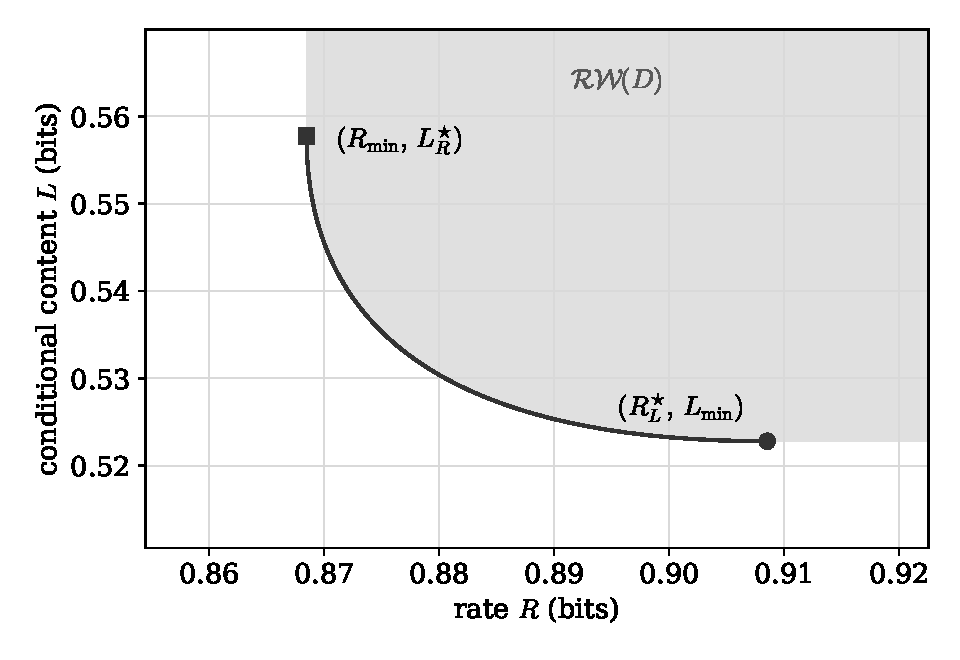
\includegraphics[width=\columnwidth]{frontier}
\caption{The Pareto frontier of the rate--content region at
$(\rho^2,\tau^2,D)=(0.75,0.5,0.3)$, traced by the two-water-level system of
Theorem~\ref{thm:region}. The tradeoff is strict: the rate-optimal channel
pays $\LRs(D)-L(D)=0.0349$ bits of excess conditional content, and the
content-optimal channel pays $\RLs(D)-R_{\min}=0.0400$ bits of excess
rate.}
\label{fig:frontier}
\end{figure}

\begin{figure}[!t]
\centering

\includegraphics[width=\columnwidth]{frontier_multi}
\caption{The frontier at three correlations, fixed $(\tau^2,D)=(0.5,0.3)$.
The endpoint gap between the rate-optimal and content-optimal channels
widens from $\rho^2=0.2$ ($\Delta R=0.021$, $\Delta L=0.017$ bits) to
$\rho^2=0.5$ ($\Delta R=0.044$, $\Delta L=0.036$) and eases at
$\rho^2=0.8$ ($\Delta R=0.035$, $\Delta L=0.031$): the tradeoff vanishes at
$\rho^2=0$, is widest at intermediate misalignment, and closes again toward
the $\rho^2\to1$ boundary. Marker shape distinguishes the curves; the gaps
are printed by the plotting script.}
\label{fig:frontiermulti}
\end{figure}

\begin{remark}[The tradeoff persists at the clean-context boundary]
\label{rem:cleanboundary}
The strict tradeoff extends to the boundary $\tau^2=0$ excluded by the
standing model. Let $\tau^2=0$, so $S=V$, and let $\rho^2\in(0,1)$,
$0<D<1$. The minimal conditional content is
\begin{equation}
L_{\min}(D)\;=\;\tfrac12\log_2^{+}\frac{1-\rho^2}{D},
\label{eq:cleanmin}
\end{equation}
while \emph{every} channel attaining the minimal rate
$R_{\min}=\tfrac12\log_2(1/D)$, in particular the classical reverse
channel $\hY_R=(1-D)Y+N$ with $N\sim\mathcal N(0,D(1-D))$ independent
of $X$, has conditional content exactly
\begin{equation}
\LRs(D)\;=\;\tfrac12\log_2\frac{(1-D)(1-\rho^2)+D}{D}
\;=\;\tfrac12\log_2\frac{1-\rho^2+D\rho^2}{D}\;>\;L_{\min}(D),
\label{eq:cleanrev}
\end{equation}
strictly, on all of $0<D<1$. In particular no channel attains
$R_{\min}$ and $L_{\min}$ simultaneously: a clean context trades rate
against content just as a noisy one does, for $D<1-\rho^2$ with both
quantities positive, and for $D\ge1-\rho^2$ with $L_{\min}=0$ but
$\LRs>0$.
\end{remark}

\begin{proof}
\emph{The value \eqref{eq:cleanmin}.} Write $Y=\rho V+Y'$ with
$Y'\perp V$, $\operatorname{Var}Y'=1-\rho^2$. Converse: for any
admissible channel, $I(X;\hY\mid V)\ge I(Y;\hY\mid V)\ge R_{Y\mid
V}(D)=\tfrac12\log_2^{+}\bigl(\operatorname{Var}(Y\mid
V)/D\bigr)$, Gray's conditional function \cite{gray1973}, exactly as
in Proposition~\ref{prop:marg}(ii). Achievability for $D\le1-\rho^2$:
with $\theta=D/(1-\rho^2)$, take
$\hY=\rho V+(1-\theta)Y'+N$, $N\sim\mathcal
N\bigl(0,\theta(1-\theta)(1-\rho^2)\bigr)$: the distortion is
$\theta^2(1-\rho^2)+\theta(1-\theta)(1-\rho^2)=D$, and
\[
I(T;\hY\mid V)
=\tfrac12\log_2
\frac{\operatorname{Var}(\hY\mid V)}{\operatorname{Var}(\hY\mid T)}
=\tfrac12\log_2
\frac{(1-\theta)^2(1-\rho^2)+\theta(1-\theta)(1-\rho^2)}
{\theta(1-\theta)(1-\rho^2)}
=\tfrac12\log_2\frac{1-\rho^2}{D}\,.
\]
For $D\ge1-\rho^2$, $\hY=\rho V$ has distortion $1-\rho^2\le D$ and is
$V$-measurable, so $I(T;\hY\mid V)=0$.

\emph{The value \eqref{eq:cleanrev}.} For the reverse channel,
$\operatorname{Var}(\hY_R\mid V)=(1-D)^2\operatorname{Var}(Y\mid
V)+\operatorname{Var}N=(1-D)^2(1-\rho^2)+D(1-D)$ and
$\operatorname{Var}(\hY_R\mid T)=\operatorname{Var}N=D(1-D)$, so
\[
\LRs(D)=\tfrac12\log_2
\frac{(1-D)^2(1-\rho^2)+D(1-D)}{D(1-D)}
=\tfrac12\log_2\frac{(1-D)(1-\rho^2)+D}{D}\,,
\]
and $(1-D)(1-\rho^2)+D=1-\rho^2+D\rho^2$.

\emph{Every rate-optimal channel carries the content
\eqref{eq:cleanrev}.} The rate moment program never references the
conditioner, and at $\alpha=1$ the uniqueness proof of
Proposition~\ref{prop:uniq} is $\Lambda$-free (the closing note
there), so also at $\tau^2=0$ its unique minimizer is
$(a,b,\nu)=(1-D,0,D(1-D))$. Let a channel attain $R_{\min}$ at
distortion $D$. The chain
$R_{\min}=I(T;\hY)\ge B_0(\text{its moments})\ge\min B_0=R_{\min}$
forces its moments to be that triple and forces equality in the
max-entropy bound \eqref{eq:lem-rate}. Equality makes the
linear-estimation error $E:=T-J\hY$,
$J=\E[T\hY]/\operatorname{Var}\hY$, Gaussian and independent of
$\hY$. At these moments $\operatorname{Var}\hY=(1-D)^2+D(1-D)=1-D$
and $\E[Y\hY]=1-D$, so the $Y$-row of $J$ is $1$ and
$Y=\hY+E_Y$ with $E_Y$ Gaussian independent of $\hY$ and $Y$ standard
Gaussian; by Cram\'er's decomposition theorem \cite{cramer1936},
$\hY$ is Gaussian. Independent Gaussian vectors are jointly Gaussian,
so $(T,\hY)=(J\hY+E,\hY)$ is jointly Gaussian with the pinned
moments: the law of the reverse channel. Its conditional content is
then determined by that law,
\[
I(T;\hY\mid V)
=\tfrac12\log_2
\frac{\operatorname{Var}(\hY\mid V)}{\operatorname{Var}(\hY\mid T)}
=\tfrac12\log_2\frac{(1-D)-(1-D)^2\rho^2}{D(1-D)}
=\tfrac12\log_2\frac{1-\rho^2+D\rho^2}{D}\,,
\]
which is \eqref{eq:cleanrev}.

\emph{Strictness.} For $D<1-\rho^2$:
$1-\rho^2+D\rho^2>1-\rho^2$ since $D\rho^2>0$, so $\LRs>L_{\min}$. For
$1-\rho^2\le D<1$: $L_{\min}=0$, while
$1-\rho^2+D\rho^2>D\Leftrightarrow(1-\rho^2)(1-D)>0$, so $\LRs>0$.
\end{proof}

\begin{corollary}[$L$ is not determined by the reduced marginal $(Y,S)$]
\label{cor:notmarginal}
Two instances whose $(Y,S)$ joint laws are equivalent up to bijective
scaling can have different minimal conditional content: the instances
$(\rho^2,\tau^2)=(\tfrac12,0)$ and $(\tfrac34,\tfrac12)$ have
$\rho_{YS}^2=\tfrac12$ in both cases, yet different $L$ at both tested
distortions; Table~\ref{tab:notmarginal} lists the values, both
strictly below Steinberg's scalar formula evaluated on the reduced pair.
So no functional of the $(Y,S)$
joint law, in particular neither Steinberg's scalar formula evaluated on
$(Y,S)$ nor Gray's, can equal $L$. This is no departure from Steinberg's
functional, whose source here is the full pair $(Y,V)$; it shows the
augmentation is essential: the encoder's access to the clean context
$V$ enters the function.
\end{corollary}

\begin{table}[!t]
\caption{The values behind Corollary~\ref{cor:notmarginal}: two
instances with the same reduced $(Y,S)$ law ($\rho_{YS}^2=\tfrac12$),
in bits. The two $L$ rows differ at both distortions, and both lie
below the Steinberg row. Exact forms for the second instance:
$g^\star=(17+\sqrt{229})/6$ at $D=0.1$ and $(21+\sqrt{261})/18$ at
$D=0.3$ (displayed in the proof).}
\label{tab:notmarginal}
\centering
\footnotesize
\begin{tabular}{lccc}
\hline
 & $\operatorname{Corr}(Y,S)=\rho/\sqrt{s}$ & $L$ at $D=0.1$ & $L$ at $D=0.3$\\
\hline
Instance $(\rho^2,\tau^2)=(\tfrac12,0)$ & $1/\sqrt2$ & $1.1610$ & $0.3685$\\
Instance $(\rho^2,\tau^2)=(\tfrac34,\tfrac12)$ & $1/\sqrt2$ & $1.2105$ & $0.5228$\\
Steinberg's scalar formula on the reduced pair & $1/\sqrt2$ & $1.2297$ & $0.5577$\\
\hline
\end{tabular}
\end{table}


\begin{proof}
The two instances share the $(Y,S)$ joint law: in both, $Y$ is standard
and
$\rho_{YS}^2=\Cov(Y,S)^2/\operatorname{Var}S=\rho^2/s$ equals
$\tfrac12$, namely $(\tfrac12)/1$ and $(\tfrac34)/(\tfrac32)$, and
rescaling $S$ changes none of the quantities considered: a bijective
scaling $S\mapsto\kappa S$, $\kappa\ne0$, leaves the generated
$\sigma$-algebra unchanged, $\sigma(\kappa S)=\sigma(S)$, so every
conditional mutual information given $S$, and with it $L(D)$, is
invariant, and the two instances may be normalized to a common
$(Y,S)$ law.

\emph{First instance,} $(\rho^2,\tau^2)=(\tfrac12,0)$: the context is
clean. This instance sits at the boundary $\tau^2=0$ excluded by the
standing assumption $\tau^2>0$ of Section~\ref{sec:pair}, so its value
is supplied not by Theorem~\ref{thm:function} but directly by
Proposition~\ref{prop:marg}(ii), which is proved at $\tau^2=0$ (and
which the $\tau^2\to0$ anchor of Corollary~\ref{cor:anchors} matches
in the limit). The instance gives
\[
L=\tfrac12\log_2\frac{1}{2D}\,,
\]
so $L=\tfrac12\log_2 5=1.1610$ bits
at $D=0.1$, and $L=\tfrac12\log_2(5/3)=0.3685$ bits at $D=0.3$.

\emph{Second instance,} $(\rho^2,\tau^2)=(\tfrac34,\tfrac12)$:
$s=\tfrac32$, and \eqref{eq:Pg} becomes, at $D=0.1$,
\[
P(g)=\tfrac{3}{20}g^2-\tfrac{17}{20}g+\tfrac14,
\qquad
g^\star=\frac{17+\sqrt{229}}{6}=5.3555,
\qquad
L=\tfrac12\log_2 g^\star=1.2105\ \text{bits},
\]
and, at $D=0.3$,
\[
P(g)=\tfrac{9}{20}g^2-\tfrac{21}{20}g+\tfrac14,
\qquad
g^\star=\frac{21+\sqrt{261}}{18}=2.0642,
\qquad
L=\tfrac12\log_2 g^\star=0.5228\ \text{bits}.
\]

\emph{The value of Steinberg's scalar formula on the reduced pair:} an
encoder observing $Y$
alone pays the marginalized-class optimum of
Section~\ref{sec:function}, the scalar-corner value
$\tfrac12\log_2\bigl[(1-\rho_{YS}^2+\rho_{YS}^2D)/D\bigr]$ at
$\rho_{YS}^2=\tfrac12$, that is,
$\tfrac12\log_2\bigl[(1+D)/(2D)\bigr]$: $\tfrac12\log_2 5.5=1.2297$
bits at $D=0.1$, and $\tfrac12\log_2(13/6)=0.5577$ bits at $D=0.3$.
Both instances lie strictly below it ($1.1610,\,1.2105<1.2297$ and
$0.3685,\,0.5228<0.5577$), as Proposition~\ref{prop:marg} requires.

Since the two instances have the same $(Y,S)$ law after this
normalization and different $L$, no functional of the $(Y,S)$ joint
law, in particular neither Steinberg's scalar formula evaluated on the
pair nor Gray's under any reparameterization, can equal $L$.
\end{proof}

The mechanism is worth stating plainly. Both instances have the same
reduced correlation $\operatorname{Corr}(Y,S)=\rho/\sqrt{s}=1/\sqrt2$,
realized by different splits: entirely through a clean context in the
first instance ($\rho^2=\tfrac12$, $\tau^2=0$), through a stronger
context read in noise in the second ($\rho^2=\tfrac34$,
$\tau^2=\tfrac12$). The function depends on $(\rho^2,\tau^2)$
separately, not only through the ratio $\rho^2/s$, because the
encoder's channel acts on its observation of $(Y,V)$, not on $(Y,S)$:
two sources with identical $(Y,S)$ joint laws but different internal
splits of the correlation admit different optimal channels.
The gap at the tabulated levels is $0.0495$ bits at $D=0.1$ and
$0.1543$ bits at $D=0.3$.

\begin{remark}[Determinant-bound attainment]\label{rem:floor}
The result of this remark is stated without proof; the proof, which
tracks equalities through the entropy chain behind the bound and treats
the clean-context branch through a Cram\'er-decomposition lemma, is in
the archived full-length version of this paper at the repository record
of the title footnote. Let $Y=(Y_A,Y_B)$ be a pair of normalized
described variables with individual constraints
$\Delta=\mathrm{diag}(D_A,D_B)\succ0$, $\beta=\Cov(Y,V)$,
$\Sigma_{Y\mid V}=\Sigma_Y-\beta\beta^{\mathsf T}$, and
$\Sigma_{Y\mid S}=\Sigma_Y-\beta\beta^{\mathsf T}/s$. Every admissible
joint channel obeys the determinant lower bound
$L\ge\Bdet:=\tfrac12\log_2\bigl(\det\Sigma_{Y\mid S}/\det\Delta\bigr)$,
the conditional analogue of the Hadamard-type rate bound whose
unconditional tightness was settled by Chen et al.\ \cite{chen2026}. The
bound is attained iff (a) $\tau^2=0$ and $\Delta\preceq\Sigma_{Y\mid V}$,
or (b) $\beta=0$ and $\Delta\preceq\Sigma_Y$; on the misaligned branch
$\tau^2>0$, $\beta\ne0$, it is strict at every positive $(D_A,D_B)$,
with a deficit of order $\|\Delta\|$ as $\Delta\to0$. The covariance
that carries the condition is the encoder-accessible $\Sigma_{Y\mid V}$,
not the third party's $\Sigma_{Y\mid S}$, the same substitution as in
Proposition~\ref{prop:marg}. For a single described variable the
statement can be read off the closed form: on
$D\le\operatorname{Var}(Y\mid V)=1-\rho^2$ the bound
$\tfrac12\log_2\bigl(\operatorname{Var}(Y\mid S)/D\bigr)$ is attained
iff $\rho\tau=0$, since substituting $g_f=(s-\rho^2)/(Ds)$ into the
quadratic \eqref{eq:Pg} gives $P(g_f)=-\rho^2\tau^2/s$, which is
negative, so that $g^\star>g_f$ strictly, exactly when $\rho\tau\ne0$.
\end{remark}

\section{Vector Context}
\label{sec:vector}

The frontier survives a vector conditioner. Let
$S=\Gamma^{\mathsf T}X+U\in\R^r$, $U\sim\mathcal N(0,\Sigma_U)$,
$\Sigma_U\succ0$, with $X$, $U$, and all channel randomness mutually
independent. Write $V:=\Gamma^{\mathsf T}X\in\R^r$ and
$T:=(Y,V)\in\R^{1+r}$, and assume $\Sigma_T\succ0$; degenerate
instances reduce by dropping linearly dependent context components.
Reproductions are scalar without loss of optimality by the
data-processing reduction of Section~\ref{sec:pair}, which is generic
in $S$.

\begin{theorem}[Vector context]\label{thm:vector}
Let $0<D<1$.
(i) \emph{Sufficiency:} it is without loss of optimality to let the
channel depend on $X$ only through $T$, and then
$I(X;\hY\mid S)=I(T;\hY\mid S)$.
(ii) \emph{Whitened form:} with $W$, $Z=WT$,
$\Lambda=\mathrm{diag}(\lambda_1,\dots,\lambda_{1+r})$,
$0\prec\Lambda\preceq I$, and the unit vector $y_0$ of
\eqref{eq:whitening} at $p=1+r$, every admissible channel with
regression vector $c=\E[Z\hY]$ and residual variance $\nu>0$ satisfies
\begin{equation}
R\ \ge\ \tfrac12\log_2\frac{|c|^2+\nu}{\nu},
\qquad
L\ \ge\ \tfrac12\log_2\frac{c^{\mathsf T}\Lambda c+\nu}{\nu},
\qquad
\E(Y-\hY)^2=|y_0-c|^2+\nu,
\label{eq:vec-bounds}
\end{equation}
with both bounds attained simultaneously by the jointly Gaussian
channel $\hY=c^{\mathsf T}Z+N$, $N\sim\mathcal N(0,\nu)$.
(iii) \emph{The frontier}, traced by $\alpha\in[0,1]$: with
$\gamma_0=\nu/(|c|^2+\nu)$ and
$\gamma_1=\nu/(c^{\mathsf T}\Lambda c+\nu)$, the Pareto-optimal channel is
the unique solution with $\nu>0$ of the generalized two-water-level
system
\begin{equation}
c=\bigl(1-\alpha\gamma_0-(1-\alpha)\gamma_1\bigr)
\bigl[\bigl(1-(1-\alpha)\gamma_1\bigr)I
+(1-\alpha)\gamma_1\Lambda\bigr]^{-1}y_0,
\qquad
\nu=D-|y_0-c|^2,
\label{eq:vecfoc}
\end{equation}
per-mode explicit given the two scalars $(\gamma_0,\gamma_1)$, and the
frontier point is
$\bigl(\tfrac12\log_2(1/\gamma_0),\,\tfrac12\log_2(1/\gamma_1)\bigr)$.
For $r=1$ the program coincides with that of Theorem~\ref{thm:region}
under the linear bijection $c=W^{-\mathsf T}(a,b)^{\mathsf T}$, so the
two systems trace the same frontier. The $\alpha=0$ endpoint gives the
vector-context function $L(D)$ as a one-dimensional root problem in
$\gamma_1$.
\end{theorem}

\begin{proof}
(i) In the resampling proof of Theorem~\ref{thm:pair}, the only
property of $S$ used is that its conditional law given $(X,\hY)$, and
given $(X,\hY')$, is the fixed kernel
$p(s\mid t,\hat y)=p_U(s-v)$, depending on $x$ only through $t$. This
holds verbatim for the vector $S=V+U$ with
$U\sim\mathcal N(0,\Sigma_U)$ jointly independent of $X$ and the
channel randomness. Steps (a) through (d) of that proof are unchanged.

(ii) \emph{Whitening.} First,
$\Sigma_{T\mid S}=\Sigma_T-\Sigma_{TS}\Sigma_S^{-1}\Sigma_{ST}\succ0$,
where $\Sigma_S=\Sigma_V+\Sigma_U$ is the conditioner's covariance
($V$ is not renormalized in this section):
positivity of $\Cov(T,S)$ holds because $\Sigma_T\succ0$ and
$\Sigma_{S\mid T}=\Cov(\Gamma^{\mathsf T}X\mid T)+\Sigma_U\succeq
\Sigma_U\succ0$, and the Schur complement of a positive definite
matrix is positive definite. Also $\Sigma_{T\mid S}\preceq\Sigma_T$.
The congruence \eqref{eq:whitening} therefore exists at $p=1+r$ with
$0\prec\Lambda\preceq I$, and $\Cov Z=I$ makes $y_0$ a unit vector:
$Y=y_0^{\mathsf T}Z$, $|y_0|^2=e_Y^{\mathsf T}\Sigma_Te_Y=1$.

\emph{Moments and the two bounds.} Fix an admissible channel, centered
without loss, with $c=\E[Z\hY]$ and
$\nu=\operatorname{Var}\hY-|c|^2$; the case $\nu=0$ is dispatched by
Remark~\ref{rem:degenerate} (the reproduction is then a noiseless
linear functional of $T$, so either every bound is trivial or the
reproduction is null). The residual $N'=\hY-c^{\mathsf T}Z$ is
uncorrelated with $Z$, hence with $T$ and with its subvector $V$; and
it is uncorrelated with $U$ by mutual independence, hence with
$S=V+U$: componentwise, $\Cov(N',S)=0$. Lemma~\ref{lem:gauss} (the two
determinant lower bounds, with equality for the jointly Gaussian
channel matching the second moments) applies with $A=c^{\mathsf T}W$:
$A\Sigma_TA^{\mathsf T}=c^{\mathsf T}W\Sigma_TW^{\mathsf T}c=|c|^2$
and
$A\Sigma_{T\mid S}A^{\mathsf T}=c^{\mathsf T}\Lambda c$, giving the
two bounds of \eqref{eq:vec-bounds}. The distortion evaluation is
exact because $Z$ is white:
$\E(Y-\hY)^2=1-2y_0^{\mathsf T}c+(|c|^2+\nu)=|y_0-c|^2+\nu$. Equality for
the Gaussian channel is Lemma~\ref{lem:gauss}'s equality clause.

(iii) \emph{The weighted program.} As in
Theorem~\ref{thm:region}: both coordinates are convex in the channel,
so the frontier is the trace of the weighted minimizations, and the
weighted objective is bounded below by the moment program
\[
\min_{c,\nu}\
\frac\alpha2\log_2\frac{Q_0+\nu}{\nu}
+\frac{1-\alpha}2\log_2\frac{Q_1+\nu}{\nu},
\qquad
Q_0=|c|^2,\quad
Q_1=c^{\mathsf T}\Lambda c,\quad
|y_0-c|^2+\nu\le D,\ \nu>0,
\]
whose value the Gaussian channel of (ii) attains. The objective is
strictly decreasing in $\nu$ at fixed $c\ne0$, so the distortion
constraint is active at the optimum. Feasibility forces
$2y_0^{\mathsf T}c\ge1-D+(|c|^2+\nu)>1-D>0$ as in \eqref{eq:cnonzero}, so
$c\ne0$ and $Q_1\ge\lambda_{\min}|c|^2$ is bounded away from zero on
the feasible set, giving coercivity as $\nu\to0$ and attainment at an
interior stationary point of the reduced objective in $c$, with
$\nu=D-|y_0-c|^2$.

\emph{The first-order system.} At such a point, with
$h=|y_0-c|^2$, $\nabla h=-2(y_0-c)$, $\nabla \nu=2(y_0-c)$,
$\nabla Q_0=2c$, and $\nabla Q_1=2\Lambda c$, stationarity of
$\alpha\ln(Q_0+\nu)+(1-\alpha)\ln(Q_1+\nu)-\ln \nu$ reads, after
multiplying by $\nu/2$,
\[
\alpha\gamma_0\bigl(c+(y_0-c)\bigr)
+(1-\alpha)\gamma_1\bigl(\Lambda c+(y_0-c)\bigr)
-(y_0-c)=0 .
\]
The first parenthesis collapses, $c+(y_0-c)=y_0$; collecting the $c$
terms,
\[
\bigl[\bigl(1-(1-\alpha)\gamma_1\bigr)I
+(1-\alpha)\gamma_1\Lambda\bigr]c
=\bigl(1-\alpha\gamma_0-(1-\alpha)\gamma_1\bigr)y_0,
\]
which is \eqref{eq:vecfoc}. The bracket is invertible: each diagonal
entry $\bigl(1-(1-\alpha)\gamma_1\bigr)+(1-\alpha)\gamma_1\lambda_j$
is a convex combination of $1$ and $\lambda_j>0$, since
$(1-\alpha)\gamma_1\in[0,1)$. Uniqueness of the minimizer, and hence
of the system's solution with $n>0$, at every $\alpha\in[0,1]$ is
Proposition~\ref{prop:uniq} at $p=1+r$ (the weighted program is convex
in the moment coordinates with a unique minimizer, and every
stationary point with $n>0$ is that minimizer); its proof is
dimension-free.
Achievability of the frontier point is (ii).

For $r=1$ the bijection $c=W^{-\mathsf T}(a,b)^{\mathsf T}$ carries
$(Q_0,Q_1,h)$ and the constraint to their Section~\ref{sec:function}
forms, so the two weighted programs are identical with the same unique
minimizer, and the two stationarity systems are equivalent
parameterizations of it. At $\alpha=0$, \eqref{eq:vecfoc} reads
$c=(1-\gamma_1)\bigl[(1-\gamma_1)I+\gamma_1\Lambda\bigr]^{-1}y_0$;
substituting into $n=D-|y_0-c|^2$ and
$\gamma_1=n/(c^{\mathsf T}\Lambda c+n)$ leaves one scalar equation in
$\gamma_1\in(0,1)$, the vector-context generalization of the
quadratic \eqref{eq:Pg}.
\end{proof}

\section{The Binary Solution}
\label{sec:binary}

The binary case is in this paper for two reasons: it shows that the
misalignment phenomenon and the strict rate--content tradeoff are not
Gaussian artifacts, the frontier being fully characterized here too
(Remark~\ref{rem:binfrontier}), and it shows the functional is
explicitly computable outside the Gaussian family. The case closes
completely and, unlike its Gaussian counterpart, with an elementary
self-contained proof.

Let $(Y,V)$ be a doubly symmetric binary pair (fair marginals,
$\Pr[Y\ne V]=p\in(0,\tfrac12)$), context $V$, side information
$S=V\oplus W$ with $W\sim\mathrm{Bern}(q)$, $q\in[0,\tfrac12]$,
independent. The description is the reproduction $\hY\in\{0,1\}$ itself
(richer descriptions only cost more: for any stored $Z$ from which the
decoder computes $\hY=f(Z)$, $I(Y,V;Z\mid S)\ge I(Y,V;\hY\mid S)$
by the data-processing inequality), and the distortion is Hamming,
$\Pr[\hY\ne Y]\le D$. Write $x*q=x(1-q)+(1-x)q$,
$\ell(x)=\ln\frac{1-x}{x}$, and $h_2$ for the binary entropy function
in bits.

\begin{lemma}[Convexity over the shared channel]\label{lem:binconvex}
$L(C):=I(Y,V;\hY\mid S)$ is convex in the channel
$C=P(\hat y\mid y,v)$, and the Hamming distortion is linear in $C$.
\end{lemma}

\begin{proof}
The Markov chain $\hY-(Y,V)-S$ means that one channel $C$ is shared
across the values of $S$, so $L(C)=\sum_sP(s)\,I_s(C)$, where $I_s(C)$
is the mutual information of the channel $C$ under the input law
$P(Y,V\mid S=s)$. The input laws depend on $s$, but each $I_s$ is
convex in $C$ at its own fixed input law, so the nonnegative
combination is convex in $C$. Linearity of the distortion is immediate.
\end{proof}

\begin{lemma}[The tilt root: existence, interiority, uniqueness]
\label{lem:tiltroot}
Fix $p\in(0,\tfrac12)$, $q\in(0,\tfrac12]$, $D\in(0,\tfrac12)$.
Parameterize the constraint segment $(1-p)d_0+pd_1=D$,
$(d_0,d_1)\in(0,1)^2$, by
$d_0\in\bigl(\max\{0,\tfrac{D-p}{1-p}\},\ \tfrac{D}{1-p}\bigr)$, an
open subinterval of $(0,1)$, and define the tilt residual
\[
\psi(d_0):=\ell(d_0)-\ell\bigl(d_1(d_0)\bigr)
-2(1-2q)\,\ell\bigl(u(d_0)\bigr),
\]
\[
d_1(d_0)=\frac{D-(1-p)d_0}{p},\qquad
u=a*q,\qquad a=2(1-p)d_0+p-D .
\]
Then $\psi$ has exactly one zero on the open segment, and the family
value $L(d_0)$ attains its minimum over the closed segment exactly
there. The same statements hold at $q=0$ when $D<p$.
\end{lemma}

\begin{proof}
Work in nats, with $h_e$ the binary entropy function in nats, so the
theorem's $L$ in bits is this $L$ divided by $\ln2$:
$L(d_0)=h_e(u)-(1-p)h_e(d_0)-p\,h_e\bigl(d_1(d_0)\bigr)$. Differentiating
with $h_e'(x)=\ell(x)$, $u'(d_0)=2(1-p)(1-2q)$, and $d_1'(d_0)=-(1-p)/p$,
\[
L'(d_0)=2(1-p)(1-2q)\,\ell(u)-(1-p)\,\ell(d_0)+(1-p)\,\ell(d_1)
=-(1-p)\,\psi(d_0).
\]

\emph{Existence and interiority.} We first record the boundary
behavior. At the left
endpoint: if $D\le p$ the endpoint is $d_0=0$ and
$\ell(d_0)\to+\infty$; if additionally $D=p$ then also $d_1\to1$ and
$-\ell(d_1)\to+\infty$, the same sign; if $D>p$ the endpoint is
$d_0=(D-p)/(1-p)>0$ with $d_1\to1$, so $-\ell(d_1)\to+\infty$ with the
other terms bounded. The $u$ term stays bounded in every case:
$u=a*q\in[q,1-q]$ with $q>0$. Hence $\psi\to+\infty$ at the left
endpoint. At the right endpoint $d_0=D/(1-p)<1$ (since $1-p>\tfrac12>D$):
$d_1\to0$, so $-\ell(d_1)\to-\infty$ with the other terms bounded, and
$\psi\to-\infty$. $\psi$ is continuous on the open segment, so it has a
zero there by the intermediate value theorem, and trivially every zero
is interior.

\emph{Zeros are minimizers.} The family channel is affine in
$(d_0,d_1)$, hence affine in $d_0$ along the segment, and
$L$ is convex in the channel (Lemma~\ref{lem:binconvex}), so $L$ is
convex on the segment. For
a convex differentiable function, $L'(d_0)=0$ at an interior point
makes that point a global minimizer; conversely
$L'\to-\infty$ at the left endpoint and $L'\to+\infty$ at the right
(the sign flips of $\psi$), so the minimum of $L$ over the closed
segment is attained in the interior and only at zeros of $\psi$.

\emph{Uniqueness.} The minimizer set of the convex $L$ is a closed
interval on which $L$ is constant. Suppose it contains two distinct
points. Then $L''\equiv0$ on a nondegenerate subinterval. But $L$ is
real analytic on the open segment: $d_1$ and $a$ are affine in $d_0$
with values in $(0,1)$, $u=a(1-2q)+q\in(0,1)$, and $H$ is real analytic
on $(0,1)$. By the identity theorem, $L''\equiv0$ on the whole
connected open segment, so $L'$ is constant there, contradicting
$L'\to-\infty$ at the left endpoint. Hence the minimizer is unique, and
since the zeros of $\psi$ are exactly the interior stationary points of
$L$, which are exactly its minimizers, $\psi$ has exactly one zero.

At $q=0$ with $D<p$ the same argument applies verbatim: the left
endpoint is $d_0=0$ with $d_1(0)=D/p<1$, and $u=a\in(p-D,p+D)\subset
(0,1)$ stays bounded away from $0$ and $1$, so the boundary blow-ups
and the analyticity are as before.
\end{proof}

Fig.~\ref{fig:binary} shows the objective, the tilt residual, and the
rate--content frontier at representative instances.

\begin{figure}[!t]
\centering

\includegraphics[width=0.8\columnwidth]{binary}
\caption{The binary objective $L(d_0)$ (top) and the tilt residual
$\psi(d_0)$ (middle) along the constraint segment $(1-p)d_0+pd_1=D$ at
$(p,q,D)=(0.25,0.15,0.15)$: the residual crosses zero exactly once, at
$d_0^\star=0.1173$ ($d_1^\star=0.2480$), and $L$ attains its unique
minimum $0.3346$ bits there, as Lemma~\ref{lem:tiltroot} asserts.
Bottom: the binary rate--content frontier at $(p,q,D)=(0.1,0.1,0.05)$,
the curve $\bigl(R(d_0),L(d_0)\bigr)$ along the segment
(Remark~\ref{rem:binfrontier}), with the Pareto arc from the tilt root
$d_0^\star=0.0282$ (the $L$-minimizer, $L_{\min}=0.4341$ bits) to
$d_0=D$ (the $R$-minimizer, $R_{\min}=1-h_2(D)=0.7136$ bits) drawn
bold. The tradeoff is strict: the $L$-optimal point pays
$0.0391$ bits of excess rate and the $R$-optimal point pays $0.0248$
bits of excess conditional content.}
\label{fig:binary}
\end{figure}

\begin{theorem}[The binary function]
\label{thm:binary}
For $D\in(0,\tfrac12)$, the conditional coordinate
$L(D)=\min I(Y,V;\hY\mid S)$ over channels $P(\hat y\mid y,v)$
(Markov $\hY-(Y,V)-S$) with $\Pr[\hY\ne Y]\le D$ is attained in
the two-parameter symmetric family $\hY=Y\oplus E$,
$\Pr[E=1\mid Y\oplus V=j]=d_j$, and equals
\[
L(D)\;=\;h_2(u)-(1-p)\,h_2(d_0)-p\,h_2(d_1),\qquad
u=a*q,\quad a=(1-p)d_0+p(1-d_1),
\]
where, for $q\in(0,\tfrac12]$ with any $D\in(0,\tfrac12)$, and for $q=0$
with $D<p$, the pair $(d_0,d_1)$ is the \emph{unique} solution, interior
to the constraint segment (Lemma~\ref{lem:tiltroot}), of the active
constraint $(1-p)d_0+pd_1=D$ together with the \emph{tilt equation}
\[
\ell(d_0)-\ell(d_1)\;=\;2(1-2q)\,\ell(u).
\]
At the boundary point $q=0$, $D=p$, the minimum $L=0$ is attained at
the segment endpoint $(d_0,d_1)=(0,1)$, the reproduction
$\hY=V$.
(In the excluded sliver $q=0$, $D>p$, the constraint is inactive and
$L(D)=0$, attained non-uniquely by reproductions measurable in $V$ alone; the
tilt system still has a root there, the degenerate point $d_1=1-d_0$,
which evaluates to the correct value $0$. For $q>0$ the constraint is
active on all of $(0,\tfrac12)$: $L$ is convex, nonincreasing, positive
by the last claim below, and $0$ at $D=\tfrac12$, hence strictly
decreasing.)
On the same channel the rate coordinate is $R=1-(1-p)h_2(d_0)-p\,h_2(d_1)$
and the discount is exactly $R-L=1-h_2(u)=I(\hY;S)$ (the chain-rule
identity $I(Y,V;\hY)-I(Y,V;\hY\mid S)=I(\hY;S)$, valid under the
Markov chain, in closed form: $a=\Pr[\hY\ne V]$,
$u=\Pr[\hY\ne S]$). Anchors: at $q=0$ the system gives
$a=(p-D)/(1-2D)$ and $L=h_2(p)-h_2(D)$ (Gray's conditional
rate--distortion function \cite{gray1973}, for $D\le p$); at $q=\tfrac12$
it gives $d_0=d_1=D$ and $L=1-h_2(D)$ (the marginal rate--distortion
function; the context is useless exactly when the side information is).
For $q\in(0,\tfrac12]$ and $D<\tfrac12$, $L(D)>0$.
\end{theorem}
\begin{proof}
\emph{Reduction and convexity.} Binary $\hY$ is definitional (DPI
above); convexity of $L$ in the shared channel and linearity of the
distortion are Lemma~\ref{lem:binconvex}.

\emph{Symmetrization.} The global bit flip
$\sigma:(y,v,s,\hat y)\mapsto(1{-}y,1{-}v,1{-}s,1{-}\hat y)$ preserves
the joint law of $(Y,V,S)$: the pair $(Y,V)$ is doubly symmetric with
fair marginals, so $(1{-}Y,1{-}V)\overset{d}=(Y,V)$, and $W\sim
\mathrm{Bern}(q)$ is independent of $(Y,V)$, so $S=V\oplus W$ flips
with $V$. The flip also preserves the distortion, and
$L(C^\sigma)=L(C)$;
averaging $C$ with $C^\sigma$ preserves distortion and, by convexity,
does not increase $L$. So an optimum exists among $\sigma$-symmetric
channels, and these are exactly the family $\{(d_0,d_1)\}$:
$\sigma$-symmetry forces $\Pr[\hY\ne Y\mid y,v]$ to depend only on
$y\oplus v$.

\emph{Closed form.} On the family, $H(\hY\mid Y,V)=
(1-p)h_2(d_0)+p\,h_2(d_1)$, and $\hY\oplus S=J\oplus E\oplus W$
($J=Y\oplus V$) with $\Pr[J\oplus E=1]=a$. The step
$H(\hY\mid S)=h_2(a*q)$ needs $\hY\oplus S\perp S$, which holds
because the joint law of $(\hY,S)$ is $\sigma$-invariant
($\sigma$-invariant source, $\sigma$-symmetric channel), forcing equal
conditional flip probabilities given either value of $S$; the same
symmetry gives $H(\hY)=1$, hence $R$.

\emph{Tilt equation.} Substituting $d_1=(D-(1-p)d_0)/p$ makes
$a=2(1-p)d_0+p-D$ affine in $d_0$; differentiating $L$ and using
$h_2'(x)=\ell(x)/\ln2$ and dropping the common factor $1/\ln2$ gives
$(1-p)[2(1-2q)\ell(u)-\ell(d_0)+\ell(d_1)]=0$. Since $L$ restricted to
the affine family slice is convex (restriction of a convex function),
interior stationarity is sufficient, not merely necessary.

\emph{Anchors and positivity.} $q=\tfrac12$: $u=\tfrac12$, the tilt
equation forces $d_0=d_1=D$. $q=0$: substitution of Gray's backward
channel; equality of values is elementary algebra. Positivity, in two
branches over the family (which suffices by attainment): if
$a\ne\tfrac12$, then $h_2(u)>h_2(a)\ge(1-p)h_2(d_0)+p\,h_2(1-d_1)
=(1-p)h_2(d_0)+p\,h_2(d_1)$, where the strict step holds because $u=a*q$
is strictly closer to $\tfrac12$ for $q\in(0,\tfrac12]$ and the second
step by concavity; so $L>0$. If $a=\tfrac12$, then $u=\tfrac12$,
$h_2(u)=1$, and $L=1-(1-p)h_2(d_0)-p\,h_2(d_1)\ge1-h_2(D)>0$ by
concavity at the distortion.
\end{proof}

Reproduction alphabets larger than binary are already covered by the
data-processing reduction that opens this section; no separate argument
is needed for them. The unconditional Lagrangian bounds, which assume no
convexity, numerically re-confirm that reduction and the
family-plus-tilt optimum.

\begin{remark}[The binary rate--content frontier]\label{rem:binfrontier}
The symmetric family exhausts not only the conditional coordinate but
the entire rate--content frontier at distortion $D$. The rate
coordinate $R=I(Y,V;\hY)$ is convex in the shared channel by the
argument of Lemma~\ref{lem:binconvex} with the trivial conditioner, so
every weighted objective $\alpha R+(1-\alpha)L$, $\alpha\in[0,1]$, is
convex in the channel. The global bit flip $\sigma$ of
Theorem~\ref{thm:binary}'s proof preserves the joint law of $(Y,V,S)$,
the distortion, and both coordinates: the flip is a law-preserving
bijective relabeling of both arguments of each mutual information, so
$R(C^\sigma)=R(C)$ and $L(C^\sigma)=L(C)$. Averaging a channel with its
flip therefore preserves the distortion and, by convexity, does not
increase any weighted objective, and larger reproduction alphabets are
covered by the data-processing reduction in both coordinates. Every
weighted optimum is thus attained in the family $\{(d_0,d_1)\}$, and
the distortion constraint may be taken active there: both coordinates
are nonnegative and vanish at $d_0=d_1=\tfrac12$, so by convexity the
objective does not increase along the straight path from any point
with distortion slack toward $(\tfrac12,\tfrac12)$, while the
distortion, affine in $(d_0,d_1)$ with positive weights, rises
continuously to $\tfrac12>D$ and meets the budget on the way. The
Pareto frontier of the binary rate--content region at distortion
$D$ is therefore the lower-left envelope of the curve
\[
d_0\;\longmapsto\;\bigl(R(d_0),\,L(d_0)\bigr),
\qquad
R(d_0)=1-(1-p)\,h_2(d_0)-p\,h_2\bigl(d_1(d_0)\bigr),
\]
along the constraint segment. On the segment, $R$ is strictly convex
with its unique minimum at $d_0=d_1=D$ (strict concavity of
$(1-p)h_2(d_0)+p\,h_2(d_1)$ and the stationarity
$\ell(d_0)=\ell(d_1)$), where $R=1-h_2(D)$, the marginal
rate--distortion function; $L$ has its unique minimum at the tilt root
$d_0^\star$ (Lemma~\ref{lem:tiltroot}). For $q\in(0,\tfrac12)$ the two
minimizers are distinct, since
$\psi(D)=-2(1-2q)\,\ell\bigl(u(D)\bigr)<0$ (there $u(D)<\tfrac12$
because $a(D)=p+D(1-2p)<\tfrac12$), so $d_0^\star<D$: on
$[d_0^\star,D]$ the curve is a strict tradeoff arc, $L$ increasing and
$R$ decreasing, and outside that arc both coordinates worsen. At
$q=\tfrac12$ the two minimizers coincide at $d_0=D$ and the frontier
is a single corner. Fig.~\ref{fig:binary} traces the frontier at a
representative instance.
\end{remark}

The binary conditional-content function of this paper coincides with the
common-reconstruction rate of Lu, Xu, Zhang, Feng, and Wang
\cite{lu2016lossy} (with the Heegard--Berger companion \cite{lu2016binary}),
whose encoder observes side information that may differ from the decoder's.
Under the relabeling of Appendix~\ref{app:lucompare} their function is
identically $L(D)$, so the binary $L(D)$ here is theirs; the contribution of
this section is the joint $(R,L)$ frontier they do not treat. Two further
common-reconstruction calculations are decoder-side-information ones.
Steinberg's binary example
\cite{steinberg2009} evaluates the constrained functional for a binary
symmetric pair: the decoder's side information is the source through a
binary symmetric channel, the distortion is Hamming, the optimal
reverse test channel is a BSC of crossover $D$ independent of the pair
correlation, and the value is $h_2(\rho_0*D)-h_2(D)$ at side-channel
crossover $\rho_0$. Ahmadi, Tandon, Simeone, and Poor \cite{ahmadi2013}
computed common-reconstruction functions for a binary source with
\emph{erased} side information under Hamming and erasure distortion,
in point-to-point, Heegard--Berger, and cascade configurations; the
point-to-point value is $p_e(1-h_2(D))$ at erasure rate $p_e$. Both
computations live in the decoder-side-information setting: $S$ sits at
the decoder, the encoder observes the source alone, and the
common-reconstruction constraint disciplines how the decoder may use
$S$. Theorem~\ref{thm:binary} differs structurally. Here $S$ is held
by a third party that never decodes, the encoder observes the pair
$(Y,V)$, and the constraint binds the unconditional Hamming error
$\Pr[\hY\ne Y]$. The function is anchored at Gray's conditional
function at $q=0$ and at the marginal rate--distortion function at
$q=\tfrac12$, an interpolation with no counterpart in the
decoder-side calculations. Its $q=0$ endpoint is also the
common-reconstruction value of \cite{lu2016lossy} at $p_2=0$
(Appendix~\ref{app:lucompare}). An encoder restricted to $Y$ alone faces
exactly the constrained problem of the pair $(Y,S)$, a binary
symmetric pair with crossover $p*q$, and pays Steinberg's value there
(the marginalization identity of Section~\ref{sec:function} is
alphabet-free); the tilt equation is the price of pair access.

\section{Discussion and Conclusion}
\label{sec:discussion}

This paper characterized the minimal conditional content of a description
whose encoder observes the pair $(Y,V)$ while the conditioner $S$ stays with
a third party: the closed form of Theorem~\ref{thm:function} for $Y$ and
$V$ scalar linear functionals of an arbitrary-dimensional jointly Gaussian
source, the exact rate--content region of Theorem~\ref{thm:region} with
its two-water-level frontier and the misalignment dichotomy of
Corollary~\ref{cor:misalign}, the determinant-bound attainment condition
recorded in Remark~\ref{rem:floor}, the vector-context extension of
Theorem~\ref{thm:vector}, and the complete binary solution of
Theorem~\ref{thm:binary}. The function degenerates to the classical
rate--distortion function at $\rho=0$ and to Gray's conditional function as
$\tau^2\to0$, and meets Steinberg's scalar Gaussian formula at the
$\rho^2\to1$ boundary. The structural conclusion is
Corollary~\ref{cor:notmarginal}: the function is not determined by the
reduced marginal $(Y,S)$ but by what the encoder can see, so conditional
description content is a property of the encoding configuration, not of the
source and side-information pair alone.

Under the average-work Landauer bound with side information
(Remark~\ref{rem:thermo}), $L(D)$ is exactly the minimal ideal erasure
work per symbol, in units of $\kb T\ln2$, paid by a reset mechanism that
retains $S$. The region states when storing
cheaply and erasing cheaply are compatible: at $\rho=0$ one channel minimizes
both coordinates, and under misalignment ($\rho^2\in(0,1)$, $\tau^2>0$) the
two costs strictly trade off. No result of the paper depends on this
reading: the operational theorems, the closed form, and the region are
proved without it, and Remark~\ref{rem:thermo} is the only place the
interpretation is invoked.

The same asymmetry, descriptions read by parties whose requirements they
were not sized to, extends beyond source coding. Wherever a description
is consumed under a criterion it was not sized to, the price is set by
that consumer, and the misaligned regime $\tau^2>0$ is the regime in
which the two prices separate. We claim no equivalence beyond this
correspondence of roles.

The structural conclusion also admits a broader, consumer-relative
reading. A description does not in general carry a unique operational
content independent of the configuration in which it is observed.
Reconstruction is priced by the decoder's distortion criterion.
Conditional content is priced relative to the information the reset
mechanism retains. Corollary~\ref{cor:notmarginal} makes this observer
dependence concrete within classical information theory: the reduced law
of $(Y,S)$ does not determine $L(D)$, and what the encoder can observe
matters. A companion manuscript by the author \cite{bond2026ot}
represents an observation abstractly as a triple $O=(C,G,B)$: a consumer
or observation map, an output metric, and a finite resolution budget.
The preliminary region of \cite{bond2026landauer} is stated in that
consumer-relative vocabulary. None of the results here requires the
broader formalism. They supply an operational, information-theoretic
instance of the principle it is meant to formalize: which representation
is best depends on the consumer and on the criterion under which that
consumer evaluates it.

Four problems are open. The exact rate--content region for a joint
description serving two described variables is not settled; its stationarity
system is known in necessary-condition form only. The analogous function for
a described variable of dimension greater than one is open. Stationary
sources, and the process and spectral versions of the function, are not
treated here. The finite-blocklength behavior of the pair $(R_n,L_n)$ is
unexplored, and the content coordinate is not a routine second-order
corollary of the rate one: the dispersion of $L_n$ is governed by the
variance of a conditional information density, which the
quantize-and-pass-to-the-limit argument of Appendix~\ref{app:gaussian}
does not control, so a joint $(R_n,L_n)$ dispersion region does
not follow from the rate dispersion alone.

Everything in this paper is single-letter and memoryless, Gaussian and
binary. Every closed form is verified by the independent numerical checks of
Appendix~\ref{app:numver}.

\appendices
\section{Single-Letterization}
\label{app:converse}

For completeness, we justify the last inequalities in
\eqref{eq:rate-conv} and \eqref{eq:work-conv}. For the rate coordinate,
\begin{align}
 I(X^n;\hXn)
 &=H(X^n)-H(X^n\mid\hXn)\nonumber\\
 &=\sum_{i=1}^{n}H(X_i)
   -\sum_{i=1}^{n}H(X_i\mid X^{i-1},\hXn)\nonumber\\
 &\ge\sum_{i=1}^{n}\left[H(X_i)-H(X_i\mid\hX_i)\right]\nonumber\\
 &=\sum_{i=1}^{n}I(X_i;\hX_i).
\end{align}
For the content coordinate,
\begin{align}
 I(X^n;\hXn\mid S^n)
 &=H(X^n\mid S^n)-H(X^n\mid\hXn,S^n)\nonumber\\
 &=\sum_{i=1}^{n}H(X_i\mid S_i)
   -\sum_{i=1}^{n}H(X_i\mid X^{i-1},\hXn,S^n)\nonumber\\
 &\ge\sum_{i=1}^{n}
 \left[H(X_i\mid S_i)-H(X_i\mid\hX_i,S_i)\right]\nonumber\\
 &=\sum_{i=1}^{n}I(X_i;\hX_i\mid S_i).
\end{align}

\section{The Gaussian Operational Theorem}
\label{app:gaussian}

This appendix proves the operational region theorem for the jointly
Gaussian source of Section~\ref{sec:pair}, replacing the customary
appeal to an unspecified abstract-alphabet extension. The source letter
is $X=(Y,V)$, jointly Gaussian, the pair $T$ of Section~\ref{sec:pair}
taken as the source letter, which Theorem~\ref{thm:pair} permits; the
conditioner is $S\in\R^r$ as in
Section~\ref{sec:pair} ($r=1$) or Section~\ref{sec:vector}; the
distortion is
$d(x,\hat y)=(y-\hat y)^2$, unbounded; codes, $R_n$, $D_n$, and
$L_n=H(M\mid S^n)/n$ are as in Section~\ref{sec:operational}, and
achievability is Definition~\ref{def:achievability}.

One device is fixed first, the \emph{saturating dyadic quantizers}:
for $k\ge1$, $q_k$ partitions $\R$ into the bounded cells
$[j2^{-k},(j+1)2^{-k})$, $-4^k\le j<4^k$, and the two saturating tail
cells $(-\infty,-2^k)$ and $[2^k,\infty)$, and maps each point of a
bounded cell to the cell's left endpoint and the two tail cells to
$-2^k$ and $2^k$, so that $|q_k(u)-u|\le2^{-k}+|u|\,\mathbf 1\{|u|>2^k\}$
for every real $u$. A vector is quantized coordinatewise, so its cells
are rectangles. The partitions are nested, every cell edge of $q_k$
being an edge of $q_{k+1}$, so for any random vector $Z$ the
$\sigma$-fields $\sigma(q_k(Z))$ increase with $k$, and their union
generates $\sigma(Z)$, since the dyadic rectangles generate the Borel
$\sigma$-field. Write $S_k:=q_k(S)$.

\begin{theorem}[The Gaussian operational region]\label{thm:gaussop}
For the Gaussian source under the standing assumptions of
Section~\ref{sec:pair} ($\tau^2>0$, $\Sigma_T\succ0$) and every $0<D<1$,
\[
\RW(D)=\bigcup_{p(\hat y\mid x):\,\E(Y-\hY)^2\le D}
\bigl\{(R,L):R\ge I(X;\hY),\ L\ge I(X;\hY\mid S)\bigr\},
\]
and the union is unchanged when restricted to jointly Gaussian test
channels. The nontrivial range is $0<D<1$, and the compactness step of
the proof uses $D<1$. For $D\ge1$ the result follows from the zero
reproduction, which meets the distortion constraint with $R=L=0$; the
point $D=0$ follows as the extended-real limiting case, both
coordinates diverging. Throughout, $L_n$ is a coding quantity, the
normalized conditional entropy of the stored index; its thermodynamic
reading is confined to Remark~\ref{rem:thermo}, and no step of the
proof depends on it.
\end{theorem}

\begin{proof}
\emph{Converse.} The chain of Theorem~\ref{thm:main-region}'s converse
(the discrete operational region theorem) holds verbatim with
differential entropies for the continuous source.
$M$ is discrete, so $\log|\mathcal M_n|\ge H(M)\ge I(X^n;M)\ge
I(X^n;\hY^n)$ and $H(M\mid S^n)\ge I(X^n;M\mid S^n)\ge
I(X^n;\hY^n\mid S^n)$ are unchanged. The single-letterization of
Appendix~\ref{app:converse} holds with differential entropy $h$ in place of $H$: for the
jointly Gaussian source all the differential entropies involved are
finite (the unconditional ones are Gaussian values, and each
conditional one differs from an unconditional one by a mutual
information pinned between $0$ and
$H(M)\le\log|\mathcal M_n|<\infty$, since $\hY^n$ is a function of the
finite-valued $M$), the i.i.d.\ chain rules are unchanged, and
conditioning reduces differential entropy. The per-letter induced channels satisfy the
Markov constraint by the i.i.d.\ structure, exactly as in the finite
case; the mixture channel $\bar q$ is defined by averaging the induced
conditional laws, its distortion is $D_n$, and the convexity step is
Lemma~\ref{lem:convexity} (convexity of both coordinates in the test
channel) with the per-$s$ sum replaced by the integral
against the law of $S$ (regular conditional probabilities, as in
Theorem~\ref{thm:region}'s proof). Hence
$(R_n,L_n)$ lies in the displayed union at distortion $D_n$.

\emph{Closedness and the passage from $D_n$ to $D$.} By the restriction
step below, the union at any distortion level $D'\in(0,1)$ equals the
union over jointly Gaussian test channels, and these are parameterized
by their regression vector and residual variance: in the whitened
coordinates of \eqref{eq:whitening} (the simultaneous congruence
$\Sigma_T\to I$, $\Sigma_{T\mid S}\to\Lambda$), by pairs
$\theta=(c,\nu)$ with
$Q_0=|c|^2$, $Q_1=c^{\mathsf T}\Lambda c$, distortion
$|y_0-c|^2+\nu\le D'$, and coordinates
$\bigl(\tfrac12\log_2\tfrac{Q_0+\nu}{\nu},\
\tfrac12\log_2\tfrac{Q_1+\nu}{\nu}\bigr)$. The distortion constraint
confines $\theta$ to a compact set: $|y_0-c|^2\le D'$ is a closed ball
and $0\le\nu\le D'$; and feasibility forces $c\ne0$ there, since $c=0$
gives distortion at least $|y_0|^2=1>D'$. Both coordinates are lower
semicontinuous on that set with values in $(0,\infty]$, finite and
continuous where $\nu>0$ and diverging as $\nu\to0$ at $c\ne0$. Now let
$(R_j,L_j)$ lie in the union at levels $D_j'$ with
$\limsup_jD_j'\le D$ and $(R_j,L_j)\to(R,L)$ finite. Pick feasible
$\theta_j$ whose quadrant contains $(R_j,L_j)$; the $\theta_j$
eventually lie in the compact set at level $D+\delta$ for each
$\delta>0$, so a subsequence converges to some $\theta^*$, feasible at
$D$ by continuity of the distortion in $\theta$. Lower semicontinuity
gives $\tfrac12\log_2\bigl[(Q_0+\nu)/\nu\bigr](\theta^*)\le
\liminf_j\tfrac12\log_2\bigl[(Q_0+\nu)/\nu\bigr](\theta_j)\le R$, and
likewise for the conditional coordinate, so $(R,L)$ lies in
$\theta^*$'s quadrant, hence in the union at $D$. This establishes
both closedness at fixed distortion and right-continuity in the
distortion level, and with $\limsup D_n\le D$ places every limit point
of $(R_n,L_n)$ in the union at $D$.

\emph{Restriction to Gaussian channels.} For any admissible channel,
Lemma~\ref{lem:gauss} (Gaussian exhaustion: the two determinant lower
bounds, met with equality by the jointly Gaussian channel matching the
second moments) produces the jointly Gaussian channel with the
same second moments and the same distortion, whose coordinates
$I(X;\hY)$ and $I(X;\hY\mid S)$ are componentwise no larger than the
original channel's. Its quadrant therefore
contains the original channel's quadrant, so the union over all
channels equals the union over jointly Gaussian channels. It thus
suffices to prove achievability for a jointly Gaussian test channel.

\emph{Achievability, Step A: quantizing the conditioner.} Fix a jointly
Gaussian admissible channel $p(\hat y\mid x)$ with distortion at most
$D$ and residual variance $\nu>0$ (a channel with $\nu=0$ has both
coordinates infinite, by the closedness step, and contributes nothing
to the union), and fix $\epsilon>0$. Along the saturating dyadic quantizers,
\begin{equation}
I(\hY;S_k)\;\uparrow\;I(\hY;S)\qquad(k\to\infty):
\label{eq:quant-mono}
\end{equation}
the sequence is nondecreasing because the partitions are nested (data
processing), and its supremum is $I(\hY;S)$ by monotone convergence of
mutual information under $\sigma$-fields increasing to the Borel
$\sigma$-field of $S$ \cite[Ch.~2]{pinsker1964}: mutual information is
the supremum of the mutual informations of finite measurable
partitions of the two sample spaces, and every finite Borel partition
of the $S$-space is approximated, up to sets of arbitrarily small
measure, by partitions measurable with respect to some
$\sigma(S_k)$. Choose $k$ with
\begin{equation}
I(\hY;S_\Delta)\;\ge\;I(\hY;S)-\epsilon,
\qquad S_\Delta:=S_k .
\label{eq:quant-approx}
\end{equation}
$S_\Delta$ is a function of $S$, so the Markov chain $\hY-X-S_\Delta$
holds, and by the chain-rule identity used throughout
($I(X;\hY)-I(X;\hY\mid S')=I(\hY;S')$ for any conditioner $S'$ with
$\hY-X-S'$),
\begin{equation}
I(X;\hY\mid S_\Delta)=I(X;\hY)-I(\hY;S_\Delta)
\;\le\;I(X;\hY\mid S)+\epsilon .
\label{eq:quant-chain}
\end{equation}

\emph{Achievability, Step B: discretizing the source and the
reproduction.} The pair source is now $(X,S_\Delta)$ with continuous
$X$ and finite $S_\Delta$, and the test channel is the jointly Gaussian
$p(\hat y\mid x)$. Theorem~\ref{thm:main-region} requires finite
alphabets and a bounded distortion, so we discretize both and pass to
the limit. For $m\ge1$ let $X_m:=q_m(X)$, the coordinatewise quantizer
applied to $X=(Y,V)$, and $\hY_m:=q_m(\hY)$, so that
$|\hY_m-\hY|\le2^{-m}+|\hY|\,\mathbf 1\{|\hY|>2^m\}$ and $\hY_m\to\hY$
in $L^2$. The finite-alphabet surrogate consists of the source $X_m$
and the side information $S_\Delta$ under their true joint law, which
is that of a discrete memoryless pair because $(X_m^n,S_\Delta^n)$ is a
coordinatewise function of the i.i.d.\ pairs $(X^n,S^n)$; the finite
reproduction alphabet $q_m(\R)\subset\R$; the test channel
\[
p_m(\hat y\mid x_m):=\Pr(\hY_m=\hat y\mid X_m=x_m),
\]
the conditional law of the quantized reproduction given the quantized
source; and the surrogate distortion
\[
d_m(x_m,\hat y):=\E\bigl[(Y-\hat y)^2\bigm|X_m=x_m\bigr]
=\operatorname{Var}(Y\mid X_m=x_m)+\bigl(\E[Y\mid X_m=x_m]-\hat y\bigr)^2,
\]
which is bounded, since both alphabets are finite.
Under the surrogate joint law $p(x_m,s_\Delta)\,p_m(\hat y\mid x_m)$
the Markov chain $\hY_m-X_m-S_\Delta$ holds by construction, so
Theorem~\ref{thm:main-region} applies to the surrogate and, for every
$\epsilon>0$ and every $m$, supplies a deterministic code, a function of
$X_m^n$ alone, of rate $I(X_m;\hY_m)+2\epsilon$, surrogate distortion at
most $\E_m d_m+\epsilon+o(1)$, and
\begin{equation}
H(M\mid S_\Delta^n)\;\le\;
n\bigl(I_m(X_m;\hY_m\mid S_\Delta)+3\epsilon+o(1)\bigr),
\label{eq:quant-fano}
\end{equation}
where $\E_m$ and $I_m$ are computed under the surrogate joint law; the
surrogate law of the pair $(X_m,\hY_m)$ is their true joint law, so
$I(X_m;\hY_m)$ needs no subscript. Three facts transfer these
guarantees to the original problem.

(i) \emph{The code is a code for the original source, with the same
distortion.} $X_m^n$ is a function of $X^n$, so the code is admissible
for $X^n$. Each reproduction letter $\hat y_i$ is a function of $X_m^n$,
and given $X_m^n$ the conditional law of $Y_i$ depends on $X_{m,i}$
alone, by memorylessness; hence
$\E\bigl[(Y_i-\hat y_i)^2\bigm|X_m^n\bigr]=d_m(X_{m,i},\hat y_i)$, and
taking expectations and averaging over $i$ identifies the true
distortion with the surrogate distortion.

(ii) \emph{The surrogate distortion converges to the original one.}
Since the surrogate law of $(X_m,\hY_m)$ is the true one,
\[
\E_m d_m(X_m,\hY_m)
=\E\bigl[\operatorname{Var}(Y\mid X_m)\bigr]
+\E\bigl[(\E[Y\mid X_m]-\hY_m)^2\bigr]
\;\longrightarrow\;\E(Y-\hY)^2\;\le\;D
\qquad(m\to\infty),
\]
because the nested partitions generate $\sigma(X)$, so
$\E[Y\mid X_m]\to Y$ in $L^2$ by the martingale convergence theorem,
which sends the first term to zero, and $\hY_m\to\hY$ in $L^2$.

(iii) \emph{The surrogate coordinates approach the original ones.} The
rate obeys $I(X_m;\hY_m)\le I(X;\hY)$ by data processing. For the
conditional coordinate, the chain-rule identity under the surrogate
Markov chain gives
$I_m(X_m;\hY_m\mid S_\Delta)=I(X_m;\hY_m)-I_m(\hY_m;S_\Delta)
\le I(X;\hY)-I_m(\hY_m;S_\Delta)$, so it remains to show that
$\liminf_mI_m(\hY_m;S_\Delta)\ge I(\hY;S_\Delta)$. The surrogate law of
$(\hY_m,S_\Delta)$ is
$Q_m(B\times\{j\})=\E\bigl[\Pr(\hY_m\in B\mid X_m)\,
\Pr(S_\Delta=j\mid X_m)\bigr]$, and for every bounded function $f$ on
$\R\times q_k(\R^r)$, continuous in its first argument,
\begin{align*}
\int f\,dQ_m
&=\E\Bigl[\sum_j\E\bigl[f(\hY_m,j)\bigm|X_m\bigr]\Pr(S_\Delta=j\mid X_m)\Bigr]\\
&\longrightarrow\;
\E\Bigl[\sum_j\E\bigl[f(\hY,j)\bigm|X\bigr]\Pr(S_\Delta=j\mid X)\Bigr]
=\E f(\hY,S_\Delta):
\end{align*}
$f(\hY_m,j)\to f(\hY,j)$ boundedly, the conditional expectations given
$X_m$ converge to those given $X$ by the martingale convergence theorem,
and the last equality is the conditional independence of $\hY$ and
$S_\Delta$ given $X$, the Markov chain $\hY-X-S$. So $Q_m$ converges
weakly to the true law of $(\hY,S_\Delta)$, and mutual information is
lower semicontinuous under weak convergence of the joint law
\cite{posner1975}. Hence for all large $m$,
$I_m(\hY_m;S_\Delta)\ge I(\hY;S_\Delta)-\epsilon$, and with
\eqref{eq:quant-chain},
\[
I_m(X_m;\hY_m\mid S_\Delta)\;\le\;I(X;\hY)-I(\hY;S_\Delta)+\epsilon
\;=\;I(X;\hY\mid S_\Delta)+\epsilon\;\le\;I(X;\hY\mid S)+2\epsilon .
\]

Fix $m$ so large that (ii) gives $\E_m d_m\le D+\epsilon$ and (iii)
holds. The selected code then has rate at most $I(X;\hY)+2\epsilon$,
true distortion at most $D+2\epsilon+o(1)$ by (i), and, by
\eqref{eq:quant-fano} and (iii),
\begin{equation}
H(M\mid S_\Delta^n)\;\le\;n\bigl(I(X;\hY\mid S)+5\epsilon+o(1)\bigr).
\label{eq:quant-fano2}
\end{equation}

\emph{Achievability, Step C: back to the unquantized conditioner.}
$S_\Delta^n$ is a function of $S^n$, so
$\sigma(S_\Delta^n)\subseteq\sigma(S^n)$ and conditioning on the finer
$\sigma$-algebra cannot increase entropy:
\begin{equation}
H(M\mid S^n)\;\le\;H(M\mid S_\Delta^n)
\;\le\;n\bigl(I(X;\hY\mid S)+5\epsilon+o(1)\bigr),
\label{eq:quant-back}
\end{equation}
by \eqref{eq:quant-fano2}.

\emph{Collect.} For every $\epsilon>0$ the triple
$\bigl(I(X;\hY)+2\epsilon,\ I(X;\hY\mid S)+5\epsilon,\
D+2\epsilon\bigr)$ is achievable; a diagonal sequence
$\epsilon_j\downarrow0$ of codes achieves, in the $\limsup$ sense of
Definition~\ref{def:achievability}, the corner
$\bigl(I(X;\hY),I(X;\hY\mid S)\bigr)$ at distortion $D$, and the
quadrant above the corner is immediate from the definition. Together
with the converse and the restriction step, this proves the theorem.
\end{proof}

The imports are stated for the record: monotone convergence of mutual
information under refining partitions \cite[Ch.~2]{pinsker1964} and its
lower semicontinuity under weak convergence \cite{posner1975}. Every
other step is Theorem~\ref{thm:main-region} or is proved here; no
abstract-alphabet covering or Markov lemma is invoked.

\section{Numerical Verification}
\label{app:numver}

Each closed form and each displayed matrix identity was checked
independently of the derivations, symbolically by exact computer algebra
and numerically against direct optimization over test-channel moments,
twice over: by the author's harness, written alongside the proofs, and
by a separately commissioned re-derivation, archived with the
repository. All checks pass. The core scalar algebra is
additionally machine-checked in two further engines, a Lean~4/Mathlib
module built clean with zero \texttt{sorry} and the MATLAB Symbolic
toolbox. The matrix-general exhaustion lemma, the measure-theoretic
steps (single-letterization, covering and binning, disintegration), the
matrix-convexity lemma, the uniqueness proposition, and the binary
theorem's symmetrization and positivity arguments are verified by
written proof and the numerical harnesses, not by the proof assistant.
The scripts, their archived run outputs, and the full check inventory
accompany the manuscript sources at the repository of the title
footnote (\texttt{VERIFICATION.md} in the paper directory).

\section{Comparison with the Binary Common-Reconstruction Function of Lu \emph{et al.}}
\label{app:lucompare}

Lu, Xu, Zhang, Feng, and Wang \cite{lu2016lossy} solve the binary lossy coding
problem with encoder side information and a common-reconstruction constraint;
its Heegard--Berger companion is \cite{lu2016binary}. Their model has a source
$X$, encoder side information $S_1$, and decoder side information $S_2$ forming
$X-S_1-S_2$, with the encoder observing $(X,S_1)$, the decoder reconstructing
from the message and $S_2$, and the common-reconstruction constraint that the
encoder reproduce the decoder's estimate. For the doubly symmetric binary source
with $\Pr[X\ne S_1]=p_1$ and $S_2=S_1\oplus\mathrm{Bern}(p_2)$ under Hamming
distortion, their Theorem~1 gives the achievable rate
\[
  \widetilde R^{\mathrm{CR}}(D)
  =\min_{W:\ W-(X,S_1)-S_2,\ \E d(X,f(W))\le D} I(X,S_1;W\mid S_2),
\]
evaluated in closed form in their Theorem~2.

Under the relabeling
\[
  X\leftrightarrow Y,\quad S_1\leftrightarrow V,\quad S_2\leftrightarrow S,\quad
  W\leftrightarrow\hY,\quad (p_1,p_2)\leftrightarrow(p,q),
\]
their functional is identically the conditional-content functional of
Section~\ref{sec:binary}: $I(X,S_1;W\mid S_2)=I(Y,V;\hY\mid S)$ under the same
Markov chain $\hY-(Y,V)-S$ and the same Hamming constraint, which by pair
sufficiency (Theorem~\ref{thm:pair}) is $L$. The binary conditional-content
function $L(D)$ of this paper therefore \emph{coincides} with
$\widetilde R^{\mathrm{CR}}(D)$, and we do not claim it as new. The endpoints
agree accordingly: at $q=0$ ($p_2=0$) both reduce to Gray's conditional function
$h_2(p)-h_2(D)$ (their Remark~3), the $q=0$ anchor of Theorem~\ref{thm:binary}; at
$q=\tfrac12$ ($p_2=\tfrac12$) both reduce to the marginal rate--distortion
function $1-h_2(D)$; and at $D=0$ both give $h_2(p*q)$ (their Remark~1).

The operational readings differ, and the second coordinate is new. In
\cite{lu2016lossy} the conditioning variable $S_2$ is decoder side information,
so $I(X,S_1;W\mid S_2)$ is a transmitted \emph{rate} with a Wyner--Ziv saving;
here $S$ is held by a third party that never decodes, so the same quantity is
the conditional \emph{content} $L$, while the transmitted rate is instead the
unconditional $R=I(Y,V;\hY)$, which their single-coordinate problem does not
price. The joint $(R,L)$ region and the tilt parametrization of the whole
frontier (Remark~\ref{rem:binfrontier}) have no counterpart in
\cite{lu2016lossy}: they price both coordinates of one description at once,
rather than the single common-reconstruction rate, and are the binary
contribution of this paper.

\begin{thebibliography}{99}
\bibitem{shannon1959} C. E. Shannon, ``Coding theorems for a discrete source
with a fidelity criterion,'' in \emph{IRE Nat. Conv. Rec.}, 1959, pp. 142--163.
\bibitem{berger1971} T. Berger, \emph{Rate Distortion Theory: A Mathematical
Basis for Data Compression}. Englewood Cliffs, NJ: Prentice-Hall, 1971.
\bibitem{gray1972tr} R. M. Gray, ``Conditional rate-distortion theory,''
Stanford Electronics Laboratories, Stanford, CA, Tech. Rep. 6502-2, Oct. 1972.
\bibitem{gray1973} R. M. Gray, ``A new class of lower bounds to information
rates of stationary sources via conditional rate-distortion functions,''
\emph{IEEE Trans. Inf. Theory}, vol. 19, no. 4, pp. 480--489, 1973.
\bibitem{wynerziv1976} A. D. Wyner and J. Ziv, ``The rate-distortion function
for source coding with side information at the decoder,'' \emph{IEEE Trans.
Inf. Theory}, vol. 22, no. 1, pp. 1--10, 1976.
\bibitem{pinsker1964} M. S. Pinsker, \emph{Information and Information
Stability of Random Variables and Processes}. San Francisco, CA:
Holden-Day, 1964.
\bibitem{posner1975} E. C. Posner, ``Random coding strategies for minimum
entropy,'' \emph{IEEE Trans. Inf. Theory}, vol. 21, no. 4, pp. 388--391,
1975.
\bibitem{cramer1936} H. Cram\'er, ``\"Uber eine Eigenschaft der normalen
Verteilungsfunktion,'' \emph{Math. Z.}, vol. 41, no. 1, pp. 405--414,
1936.
\bibitem{kaspi1994} A. H. Kaspi, ``Rate-distortion function when
side-information may be present at the decoder,'' \emph{IEEE Trans. Inf.
Theory}, vol. 40, no. 6, pp. 2031--2034, 1994.
\bibitem{heegardberger1985} C. Heegard and T. Berger, ``Rate distortion when
side information may be absent,'' \emph{IEEE Trans. Inf. Theory}, vol. 31,
no. 6, pp. 727--734, 1985.
\bibitem{steinberg2009} Y. Steinberg, ``Coding and common reconstruction,''
\emph{IEEE Trans. Inf. Theory}, vol. 55, no. 11, pp. 4995--5010, 2009.
\bibitem{lapidoth2014} A. Lapidoth, A. Mal\"ar, and M. Wigger, ``Constrained
source-coding with side information,'' \emph{IEEE Trans. Inf. Theory},
vol. 60, no. 6, pp. 3218--3237, 2014.
\bibitem{ahmadi2013} B. Ahmadi, R. Tandon, O. Simeone, and H. V. Poor,
``Heegard-Berger and cascade source coding problems with common reconstruction
constraints,'' \emph{IEEE Trans. Inf. Theory}, vol. 59, no. 3,
pp. 1458--1474, 2013.
\bibitem{yamamoto1997} H. Yamamoto, ``Rate-distortion theory for the Shannon
cipher system,'' \emph{IEEE Trans. Inf. Theory}, vol. 43, no. 3, pp. 827--835,
1997.
\bibitem{villard2013} J. Villard and P. Piantanida, ``Secure multiterminal
source coding with side information at the eavesdropper,'' \emph{IEEE Trans.
Inf. Theory}, vol. 59, no. 6, pp. 3668--3692, 2013.
\bibitem{schieler2014} C. Schieler and P. Cuff, ``Rate-distortion theory for
secrecy systems,'' \emph{IEEE Trans. Inf. Theory}, vol. 60, no. 12,
pp. 7584--7605, 2014.
\bibitem{tandon2013} R. Tandon, L. Sankar, and H. V. Poor,
``Discriminatory lossy source coding: Side information privacy,''
\emph{IEEE Trans. Inf. Theory}, vol. 59, no. 9, pp. 5665--5677, 2013.
\bibitem{makhdoumi2014} A. Makhdoumi, S. Salamatian, N. Fawaz, and
M. M\'edard, ``From the information bottleneck to the privacy funnel,''
in \emph{Proc. IEEE Inf. Theory Workshop (ITW)}, 2014, pp. 501--505.
\bibitem{armstrong2026} J. Armstrong, ``Source-side sufficiency for the
information bottleneck: Exact reduction and finite-block equivalence,''
arXiv:2604.26744, 2026.
\bibitem{lu2016lossy} J. Lu, Y. Xu, P. Zhang, M. Feng, and Q. Wang, ``Binary
lossy coding problem with encoder side information and common reconstruction
constraint,'' in \emph{Proc. Int. Conf. Wireless Commun. Signal Process.
(WCSP)}, 2016, pp. 1--5.
% verify page range on final (read from author PDF; DBLP was in maintenance)
\bibitem{lu2016binary} J. Lu, Y. Xu, Y. Qian, and Q. Wang, ``The binary
Heegard-Berger problem with encoder side information and common reconstruction
constraints,'' in \emph{Proc. Int. Conf. Wireless Commun. Signal Process.
(WCSP)}, 2016, pp. 1--5.
\bibitem{luxu2021} J. Lu and Y. Xu, ``Vector Gaussian Heegard-Berger problem
with common reconstructions,'' in \emph{Proc. Int. Conf. Wireless Commun. Signal
Process. (WCSP)}, 2021, pp. 1--5.
\bibitem{guler2015} B. G\"uler, E. MolavianJazi, and A. Yener, ``Remote source
coding with two-sided information,'' in \emph{Proc. IEEE Int. Symp. Inf. Theory
(ISIT)}, 2015, pp. 2176--2180.
\bibitem{meidlinger2014} M. Meidlinger, A. Winkelbauer, and G. Matz, ``On the
relation between the Gaussian information bottleneck and MSE-optimal
rate-distortion quantization,'' in \emph{Proc. IEEE Workshop Statistical Signal
Process. (SSP)}, 2014, pp. 89--92.
\bibitem{xiaoluo2005} J.-J. Xiao and Z.-Q. Luo, ``Compression of correlated
Gaussian sources under individual distortion criteria,'' in \emph{Proc. 43rd
Allerton Conf. Commun., Control, Comput.}, Monticello, IL, 2005,
pp. 438--447.
\bibitem{chen2026} S. Chen, J. Gao, Y. Shi, Y. Wu, G. Caire, H. V. Poor, and
W. Zhang, ``On the Gaussian-quadratic rate-distortion function for vector
sources with individual distortion constraints,'' \emph{IEEE Trans. Inf.
Theory}, to be published, 2026, arXiv:2607.09545.
\bibitem{lapidothtinguely2010} A. Lapidoth and S. Tinguely, ``Sending a
bivariate Gaussian over a Gaussian MAC,'' \emph{IEEE Trans. Inf. Theory},
vol. 56, no. 6, pp. 2714--2752, 2010.
\bibitem{nayak2010} J. Nayak, E. Tuncel, D. G\"und\"uz, and E. Erkip,
``Successive refinement of vector sources under individual distortion
criteria,'' \emph{IEEE Trans. Inf. Theory}, vol. 56, no. 4, pp. 1769--1781,
2010.
\bibitem{stylianou2021} E. Stylianou, C. D. Charalambous, and
T. Charalambous, ``Joint rate distortion function of a tuple of correlated
multivariate Gaussian sources with individual fidelity criteria,'' in
\emph{Proc. IEEE Int. Symp. Inf. Theory (ISIT)}, 2021, pp. 2167--2172.
\bibitem{shlezinger2019} N. Shlezinger, Y. C. Eldar, and M. R. D. Rodrigues,
``Hardware-limited task-based quantization,'' \emph{IEEE Trans. Signal
Process.}, vol. 67, no. 20, pp. 5223--5238, 2019.
\bibitem{gunduz2023} D. G\"und\"uz, Z. Qin, I. E. Aguerri, H. S. Dhillon,
Z. Yang, A. Yener, K. K. Wong, and C.-B. Chae, ``Beyond transmitting bits:
Context, semantics, and task-oriented communications,'' \emph{IEEE J. Sel.
Areas Commun.}, vol. 41, no. 1, pp. 5--41, 2023.
\bibitem{chechik2005} G. Chechik, A. Globerson, N. Tishby, and Y. Weiss,
``Information bottleneck for Gaussian variables,'' \emph{J. Mach. Learn.
Res.}, vol. 6, pp. 165--188, 2005.
\bibitem{tishby1999} N. Tishby, F. C. Pereira, and W. Bialek, ``The
information bottleneck method,'' in \emph{Proc. 37th Allerton Conf. Commun.,
Control, Comput.}, Monticello, IL, 1999, pp. 368--377.
\bibitem{landauer1961} R. Landauer, ``Irreversibility and heat generation in
the computing process,'' \emph{IBM J. Res. Dev.}, vol. 5, no. 3, pp. 183--191,
1961.
\bibitem{bennett1973} C. H. Bennett, ``Logical reversibility of computation,''
\emph{IBM J. Res. Dev.}, vol. 17, no. 6, pp. 525--532, 1973.
\bibitem{delrio2011} L. del Rio, J. \AA berg, R. Renner, O. Dahlsten, and
V. Vedral, ``The thermodynamic meaning of negative entropy,'' \emph{Nature},
vol. 474, pp. 61--63, 2011.
\bibitem{faist2015} P. Faist, F. Dupuis, J. Oppenheim, and R. Renner, ``The
minimal work cost of information processing,'' \emph{Nature Commun.}, vol. 6,
art. 7669, 2015.
\bibitem{esposito2011} M. Esposito and C. Van den Broeck, ``Second law and
Landauer principle far from equilibrium,'' \emph{Europhys. Lett.}, vol. 95,
art. 40004, 2011.
\bibitem{sagawa2012} T. Sagawa and M. Ueda, ``Fluctuation theorem with
information exchange: Role of correlations in stochastic thermodynamics,''
\emph{Phys. Rev. Lett.}, vol. 109, art. 180602, 2012.
\bibitem{parrondo2015} J. M. R. Parrondo, J. M. Horowitz, and T. Sagawa,
``Thermodynamics of information,'' \emph{Nature Phys.}, vol. 11,
pp. 131--139, 2015.
\bibitem{bond2026landauer} A. H. Bond, ``A rate--work--distortion region for
consumer-relative observation,'' preliminary manuscript, 2026, archived at
doi:10.5281/zenodo.21776291.
\bibitem{bond2026ot} A. H. Bond, ``Observation theory: Geometry,
distortion, and reliability as properties of observation,'' preprint,
Jul. 2026, archived at doi:10.5281/zenodo.21776291. % verify archive
% record on final
\end{thebibliography}

\end{document}

